% Options for packages loaded elsewhere
\PassOptionsToPackage{unicode}{hyperref}
\PassOptionsToPackage{hyphens}{url}
\PassOptionsToPackage{dvipsnames,svgnames,x11names}{xcolor}
%
\documentclass[
  letterpaper,
  DIV=11,
  numbers=noendperiod]{scrreprt}

\usepackage{amsmath,amssymb}
\usepackage{iftex}
\ifPDFTeX
  \usepackage[T1]{fontenc}
  \usepackage[utf8]{inputenc}
  \usepackage{textcomp} % provide euro and other symbols
\else % if luatex or xetex
  \usepackage{unicode-math}
  \defaultfontfeatures{Scale=MatchLowercase}
  \defaultfontfeatures[\rmfamily]{Ligatures=TeX,Scale=1}
\fi
\usepackage{lmodern}
\ifPDFTeX\else  
    % xetex/luatex font selection
\fi
% Use upquote if available, for straight quotes in verbatim environments
\IfFileExists{upquote.sty}{\usepackage{upquote}}{}
\IfFileExists{microtype.sty}{% use microtype if available
  \usepackage[]{microtype}
  \UseMicrotypeSet[protrusion]{basicmath} % disable protrusion for tt fonts
}{}
\makeatletter
\@ifundefined{KOMAClassName}{% if non-KOMA class
  \IfFileExists{parskip.sty}{%
    \usepackage{parskip}
  }{% else
    \setlength{\parindent}{0pt}
    \setlength{\parskip}{6pt plus 2pt minus 1pt}}
}{% if KOMA class
  \KOMAoptions{parskip=half}}
\makeatother
\usepackage{xcolor}
\setlength{\emergencystretch}{3em} % prevent overfull lines
\setcounter{secnumdepth}{5}
% Make \paragraph and \subparagraph free-standing
\makeatletter
\ifx\paragraph\undefined\else
  \let\oldparagraph\paragraph
  \renewcommand{\paragraph}{
    \@ifstar
      \xxxParagraphStar
      \xxxParagraphNoStar
  }
  \newcommand{\xxxParagraphStar}[1]{\oldparagraph*{#1}\mbox{}}
  \newcommand{\xxxParagraphNoStar}[1]{\oldparagraph{#1}\mbox{}}
\fi
\ifx\subparagraph\undefined\else
  \let\oldsubparagraph\subparagraph
  \renewcommand{\subparagraph}{
    \@ifstar
      \xxxSubParagraphStar
      \xxxSubParagraphNoStar
  }
  \newcommand{\xxxSubParagraphStar}[1]{\oldsubparagraph*{#1}\mbox{}}
  \newcommand{\xxxSubParagraphNoStar}[1]{\oldsubparagraph{#1}\mbox{}}
\fi
\makeatother

\usepackage{color}
\usepackage{fancyvrb}
\newcommand{\VerbBar}{|}
\newcommand{\VERB}{\Verb[commandchars=\\\{\}]}
\DefineVerbatimEnvironment{Highlighting}{Verbatim}{commandchars=\\\{\}}
% Add ',fontsize=\small' for more characters per line
\usepackage{framed}
\definecolor{shadecolor}{RGB}{241,243,245}
\newenvironment{Shaded}{\begin{snugshade}}{\end{snugshade}}
\newcommand{\AlertTok}[1]{\textcolor[rgb]{0.68,0.00,0.00}{#1}}
\newcommand{\AnnotationTok}[1]{\textcolor[rgb]{0.37,0.37,0.37}{#1}}
\newcommand{\AttributeTok}[1]{\textcolor[rgb]{0.40,0.45,0.13}{#1}}
\newcommand{\BaseNTok}[1]{\textcolor[rgb]{0.68,0.00,0.00}{#1}}
\newcommand{\BuiltInTok}[1]{\textcolor[rgb]{0.00,0.23,0.31}{#1}}
\newcommand{\CharTok}[1]{\textcolor[rgb]{0.13,0.47,0.30}{#1}}
\newcommand{\CommentTok}[1]{\textcolor[rgb]{0.37,0.37,0.37}{#1}}
\newcommand{\CommentVarTok}[1]{\textcolor[rgb]{0.37,0.37,0.37}{\textit{#1}}}
\newcommand{\ConstantTok}[1]{\textcolor[rgb]{0.56,0.35,0.01}{#1}}
\newcommand{\ControlFlowTok}[1]{\textcolor[rgb]{0.00,0.23,0.31}{\textbf{#1}}}
\newcommand{\DataTypeTok}[1]{\textcolor[rgb]{0.68,0.00,0.00}{#1}}
\newcommand{\DecValTok}[1]{\textcolor[rgb]{0.68,0.00,0.00}{#1}}
\newcommand{\DocumentationTok}[1]{\textcolor[rgb]{0.37,0.37,0.37}{\textit{#1}}}
\newcommand{\ErrorTok}[1]{\textcolor[rgb]{0.68,0.00,0.00}{#1}}
\newcommand{\ExtensionTok}[1]{\textcolor[rgb]{0.00,0.23,0.31}{#1}}
\newcommand{\FloatTok}[1]{\textcolor[rgb]{0.68,0.00,0.00}{#1}}
\newcommand{\FunctionTok}[1]{\textcolor[rgb]{0.28,0.35,0.67}{#1}}
\newcommand{\ImportTok}[1]{\textcolor[rgb]{0.00,0.46,0.62}{#1}}
\newcommand{\InformationTok}[1]{\textcolor[rgb]{0.37,0.37,0.37}{#1}}
\newcommand{\KeywordTok}[1]{\textcolor[rgb]{0.00,0.23,0.31}{\textbf{#1}}}
\newcommand{\NormalTok}[1]{\textcolor[rgb]{0.00,0.23,0.31}{#1}}
\newcommand{\OperatorTok}[1]{\textcolor[rgb]{0.37,0.37,0.37}{#1}}
\newcommand{\OtherTok}[1]{\textcolor[rgb]{0.00,0.23,0.31}{#1}}
\newcommand{\PreprocessorTok}[1]{\textcolor[rgb]{0.68,0.00,0.00}{#1}}
\newcommand{\RegionMarkerTok}[1]{\textcolor[rgb]{0.00,0.23,0.31}{#1}}
\newcommand{\SpecialCharTok}[1]{\textcolor[rgb]{0.37,0.37,0.37}{#1}}
\newcommand{\SpecialStringTok}[1]{\textcolor[rgb]{0.13,0.47,0.30}{#1}}
\newcommand{\StringTok}[1]{\textcolor[rgb]{0.13,0.47,0.30}{#1}}
\newcommand{\VariableTok}[1]{\textcolor[rgb]{0.07,0.07,0.07}{#1}}
\newcommand{\VerbatimStringTok}[1]{\textcolor[rgb]{0.13,0.47,0.30}{#1}}
\newcommand{\WarningTok}[1]{\textcolor[rgb]{0.37,0.37,0.37}{\textit{#1}}}

\providecommand{\tightlist}{%
  \setlength{\itemsep}{0pt}\setlength{\parskip}{0pt}}\usepackage{longtable,booktabs,array}
\usepackage{calc} % for calculating minipage widths
% Correct order of tables after \paragraph or \subparagraph
\usepackage{etoolbox}
\makeatletter
\patchcmd\longtable{\par}{\if@noskipsec\mbox{}\fi\par}{}{}
\makeatother
% Allow footnotes in longtable head/foot
\IfFileExists{footnotehyper.sty}{\usepackage{footnotehyper}}{\usepackage{footnote}}
\makesavenoteenv{longtable}
\usepackage{graphicx}
\makeatletter
\newsavebox\pandoc@box
\newcommand*\pandocbounded[1]{% scales image to fit in text height/width
  \sbox\pandoc@box{#1}%
  \Gscale@div\@tempa{\textheight}{\dimexpr\ht\pandoc@box+\dp\pandoc@box\relax}%
  \Gscale@div\@tempb{\linewidth}{\wd\pandoc@box}%
  \ifdim\@tempb\p@<\@tempa\p@\let\@tempa\@tempb\fi% select the smaller of both
  \ifdim\@tempa\p@<\p@\scalebox{\@tempa}{\usebox\pandoc@box}%
  \else\usebox{\pandoc@box}%
  \fi%
}
% Set default figure placement to htbp
\def\fps@figure{htbp}
\makeatother

\newcommand{\Exg}{\operatorname{\mathbb{E}}} 
\newcommand{\Ex}{\mathbb{E}} 
\newcommand{\Ind}{\mathbb{I}}
\newcommand{\Var}{\operatorname{Var}}
\newcommand{\Cov}{\operatorname{Cov}}
\newcommand{\Corr}{\operatorname{Corr}}
\newcommand{\ee}{\mathrm{e}}
\usepackage{comment}
\KOMAoption{captions}{tableheading}
\makeatletter
\@ifpackageloaded{bookmark}{}{\usepackage{bookmark}}
\makeatother
\makeatletter
\@ifpackageloaded{caption}{}{\usepackage{caption}}
\AtBeginDocument{%
\ifdefined\contentsname
  \renewcommand*\contentsname{Table of contents}
\else
  \newcommand\contentsname{Table of contents}
\fi
\ifdefined\listfigurename
  \renewcommand*\listfigurename{List of Figures}
\else
  \newcommand\listfigurename{List of Figures}
\fi
\ifdefined\listtablename
  \renewcommand*\listtablename{List of Tables}
\else
  \newcommand\listtablename{List of Tables}
\fi
\ifdefined\figurename
  \renewcommand*\figurename{Figure}
\else
  \newcommand\figurename{Figure}
\fi
\ifdefined\tablename
  \renewcommand*\tablename{Table}
\else
  \newcommand\tablename{Table}
\fi
}
\@ifpackageloaded{float}{}{\usepackage{float}}
\floatstyle{ruled}
\@ifundefined{c@chapter}{\newfloat{codelisting}{h}{lop}}{\newfloat{codelisting}{h}{lop}[chapter]}
\floatname{codelisting}{Listing}
\newcommand*\listoflistings{\listof{codelisting}{List of Listings}}
\usepackage{amsthm}
\theoremstyle{plain}
\newtheorem{theorem}{Theorem}[chapter]
\theoremstyle{definition}
\newtheorem{definition}{Definition}[chapter]
\theoremstyle{definition}
\newtheorem{example}{Example}[chapter]
\theoremstyle{remark}
\AtBeginDocument{\renewcommand*{\proofname}{Proof}}
\newtheorem*{remark}{Remark}
\newtheorem*{solution}{Solution}
\newtheorem{refremark}{Remark}[chapter]
\newtheorem{refsolution}{Solution}[chapter]
\makeatother
\makeatletter
\makeatother
\makeatletter
\@ifpackageloaded{caption}{}{\usepackage{caption}}
\@ifpackageloaded{subcaption}{}{\usepackage{subcaption}}
\makeatother

\usepackage{bookmark}

\IfFileExists{xurl.sty}{\usepackage{xurl}}{} % add URL line breaks if available
\urlstyle{same} % disable monospaced font for URLs
\hypersetup{
  pdftitle={MATH5835M Statistical Computing},
  pdfauthor={Matthew Aldridge},
  colorlinks=true,
  linkcolor={blue},
  filecolor={Maroon},
  citecolor={Blue},
  urlcolor={Blue},
  pdfcreator={LaTeX via pandoc}}


\title{MATH5835M Statistical Computing}
\author{Matthew Aldridge}
\date{2025-09-30}

\begin{document}
\maketitle

\renewcommand*\contentsname{Table of contents}
{
\hypersetup{linkcolor=}
\setcounter{tocdepth}{2}
\tableofcontents
}

\bookmarksetup{startatroot}

\chapter*{About MATH5835}\label{about-math5835}
\addcontentsline{toc}{chapter}{About MATH5835}

\markboth{About MATH5835}{About MATH5835}

\section*{Organisation of MATH5835}\label{organisation-of-math5835}
\addcontentsline{toc}{section}{Organisation of MATH5835}

\markright{Organisation of MATH5835}

This module is \textbf{MATH5835M Statistical Computing}.

This module lasts for 11 weeks from 29 September to 12 December 2025.
The exam will take place sometime between 12 and 23 January 2026.

The module leader, the lecturer, and the main author of these notes is
\href{https://mpaldridge.github.io/}{Dr Matthew Aldridge}. (You can call
me ``Matt'', ``Matthew'', or ``Dr Aldridge'', pronounced
``\emph{old}-ridge''.) My email address is
\href{mailto:m.aldridge@leeds.ac.uk}{\nolinkurl{m.aldridge@leeds.ac.uk}},
although I much prefer questions in person at office hours (see below)
rather than by email.

The HTML webpage is the best way to view the course material. There is
also a \href{MATH5835M-Statistical-Computing.pdf}{\textbf{PDF version}},
although I have been much less careful about the presentation of this
material, and it does not include the problem sheets.

\subsection*{Lectures}\label{lectures}
\addcontentsline{toc}{subsection}{Lectures}

The main way you will learn new material for this module is by attending
lectures. There are three lectures per week:

\begin{itemize}
\item
  Mondays at 1400
\item
  Thursdays at 1200
\item
  Fridays at 1000
\end{itemize}

all in in
\href{https://students.leeds.ac.uk/buildings-and-rooms/3611/roger-stevens-lt-14-10m-14}{Roger
Stevens LT 14}.

I recommend taking your own notes during the lecture. I will put brief
summary notes from the lectures on this website, but they will not
reflect all the details I say out loud and write on the whiteboard.
Lectures will go through material quite quickly and the material may be
quite difficult, so it's likely you'll want to spend time reading
through your notes after the lecture. Lectures should be recorded on the
lecture capture system; I find it very difficult to read the whiteboard
in these videos, but if you unavoidably miss a lecture, for example due
to illness, you may find they are better than nothing.

In Weeks 3, 5, 7, 9 and 11, the Thursday lecture will operate as a
``problems class'' -- see more on this below.

Attendance at lectures in compulsory. You should record your attendance
using the UniLeeds app and the QR code on the wall in the 15 minutes
before the lecture or the 15 minutes after the lecture (but not during
the lecture).

\subsection*{Problem sheets and problem
classes}\label{problem-sheets-and-problem-classes}
\addcontentsline{toc}{subsection}{Problem sheets and problem classes}

Mathematics and statistics are ``doing'' subjects! To help you learn
material for the module and to help you prepare for the exam, I will
provide 5 unassessed problem sheets. These are for you to work through
in your own time to help you learn; they are \emph{not} formally
assessed. You are welcome to discuss work on the problem sheets with
colleagues and friends, although my recommendation would be to write-up
your ``last, best'' attempt neatly by yourself.

There will be an optional opportunity to submit one or two questions
from the problem sheet to me in advance of the problems class for some
brief informal feedback on your work. See the problem sheets for
details.

You should work through each problem sheet in preparation for the
problems class in the Thursday lecture of Week 3, 5, 7, 9 and 11. In the
problems class, you should be ready to explain your answers to questions
you managed to solve, discuss your progress on questions you partially
solved, and ask for help on questions you got stuck on.

You can also ask for extra help or feedback at office hours (see below).

\subsection*{Coursework}\label{coursework}
\addcontentsline{toc}{subsection}{Coursework}

There will be one piece of assessed coursework, which will make up 20\%
of your module mark. \hyperref[coursework]{You can read more about the
coursework here.}

The coursework will be in the form of a worksheet. The worksheet will
have some questions, mostly computational but also mathematical, and you
will have to write a report containing your answers and computations.

The assessed coursework will be introduced in the \textbf{computer
practical} sessions in Week 9.

The deadline for the coursework will be the penultimate day of the
Autumn term, \textbf{Thursday 12 December } at 1400. Feedback and marks
will be returned on Monday 13 January, the first day of the Spring term.

\subsection*{Office hours}\label{office-hours}
\addcontentsline{toc}{subsection}{Office hours}

I will run a n optional ``office hours'' drop-in session each week for
feedback and consultation. You can come along if you want to talk to me
about anything on the module, including if you'd like more feedback on
your attempts at problem sheet questions. (For extremely short queries,
you can approach me before or after lectures, but my response will often
be: ``Come to my office hours, and we can discuss it there!'')

Office hours will happen on \textbf{Thursdays from 1300 to 1400} -- so
directly after the Thursday lecture / problems class -- in my office,
which is \textbf{EC Stoner 9.10n} in ``Maths Research Deck'' area on the
9th floor of the EC Stoner building. (One way to the Maths Research Deck
is via the doors directly opposite the main entrance to the School of
Mathematics; you can also get there from Staircase 1 on the Level 10
``red route'' through EC Stoner, next to the Maths Satellite.) If you
cannot make this time, contact me for an alternative arrangement.

\subsection*{Exam}\label{exam}
\addcontentsline{toc}{subsection}{Exam}

There will be one exam, which will make up 80\% of your module mark.

The exam will be in the January 2026 exam period (12--23 January); the
date and time will be announced in December. The exam will be in person
and on campus.

The exam will last 2 hours and 30 minutes. The exam will consist of 4
questions, all compulsory. You will be allowed to use a permitted
calculator in the exam.

\section*{Content of MATH5835}\label{content-of-math5835}
\addcontentsline{toc}{section}{Content of MATH5835}

\markright{Content of MATH5835}

\subsection*{Necessary background}\label{necessary-background}
\addcontentsline{toc}{subsection}{Necessary background}

I recommend that students should have completed at least two
undergraduate level courses in probability or statistics -- although
confidence and proficiency in basic material is more important than very
deep knowledge of more complicated topics.

For Leeds undergraduates, MATH2715 Statistical Methods is an official
prerequisite (please get in touch with me if you are/were a Leeds
undergraduate and have not taken MATH2715), although confidence and
proficiency in the more basic material of MATH1710 \& MATH1712
Probability and Statistics 1 \& 2 is probably more important.

Some knowledge I will assume:

\begin{itemize}
\item
  \textbf{Probability:} Basic rules of probability; random variables,
  both continuous and discrete; ``famous'' distributions (especially the
  normal distribution and the continuous uniform distribution);
  expectation, variance, covariance, correlation; law of large numbers
  and central limit theorem.
\item
  \textbf{Statistics:} Estimation of parameters; bias and error; sample
  mean and sample variance
\end{itemize}

This module will also include an material on Markov chains. I won't
assume any pre-existing knowledge of this, and I will introduce all new
material we need, but students who have studied Markov chains before
(for example in the Leeds module MATH2750 Introduction to Markov
Processes) may find a couple of lectures here are merely a reminder of
things they already know.

The lectures will include examples using the \textbf{R} program
language. The coursework and problem sheets will require use of R. The
exam, while just a ``pencil and paper'' exam, will require understanding
and writing short portions of R code. We will assume basic R capability
-- that you can enter R commands, store R objects using the
\texttt{\textless{}-} assignment, and perform basic arithmetic with
numbers and vectors. Other concepts will be introduced as necessary. If
you want to use R on your own device, I recommend downloading (if you
have not already) the \href{https://cran.r-project.org}{R programming
language} and the \href{https://posit.co/downloads/}{program RStudio}.
(These lecture notes were written in R using RStudio.)

\subsection*{Syllabus}\label{syllabus}
\addcontentsline{toc}{subsection}{Syllabus}

We plan to cover the following topics in the module:

\begin{itemize}
\item
  \textbf{Monte Carlo estimation:} definition and examples; bias and
  error; variance reduction techniques: control variates, antithetic
  variables, importance sampling. {[}9 lectures{]}
\item
  \textbf{Random number generation:} pseudo-random number generation
  using linear congruential generators; inverse transform method;
  rejection sampling {[}7 lectures{]}
\item
  \textbf{Markov chain Monte Carlo} (MCMC)\textbf{:} {[}7 lectures{]}

  \begin{itemize}
  \item
    Introduction to Markov chains in discrete and continuous space
  \item
    Metropolis--Hastings algorithm: definition; examples; MCMC in
    practice; MCMC for Bayesian statistics
  \end{itemize}
\item
  \textbf{Resampling methods:} Empirical distribution; plug-in
  estimation; bootstrap statistics; bootstrap estimation {[}4
  lectures{]}
\item
  Frequently-asked questions {[}1 lecture{]}
\end{itemize}

Together with the 5 problems classes, this makes 33 lectures.

\subsection*{Book}\label{book}
\addcontentsline{toc}{subsection}{Book}

The following book is strongly recommended for the module:

\begin{itemize}
\tightlist
\item
  J Voss,
  \href{https://leeds.primo.exlibrisgroup.com/permalink/44LEE_INST/1fj430b/cdi_askewsholts_vlebooks_9781118728031}{\emph{An
  Introduction to Statistical Computing: A simulation-based approach}},
  Wiley Series in Computational Statistics, Wiley, 2014
\end{itemize}

The library has
\href{https://leeds.primo.exlibrisgroup.com/permalink/44LEE_INST/1fj430b/cdi_askewsholts_vlebooks_9781118728031}{electronic
access to this book} (and two paper copies).

Dr Voss is a lecturer in the School of Mathematics and the University of
Leeds, and has taught MATH5835 many times. \emph{An Introduction to
Statistical Computing} grew out of his lecture notes for this module, so
the book is ideally suited for this module. My lectures will follow this
book closely -- specifically:

\begin{itemize}
\item
  Monte Carlo estimation: Sections 3.1--3.3
\item
  Random number generation: Sections 1.1--1.4
\item
  Markov chain Monte Carlo: Section 2.3 and Sections 4.1--4.3
\item
  Bootstrap: Section 5.2
\end{itemize}

For a second look at material, for preparatory reading, for optional
extended reading, or for extra exercises, this book comes with my
highest recommendation!

\part{Monte Carlo estimation}

\chapter{Introduction to Monte Carlo}\label{introduction-to-monte-carlo}

\[ \]

Today, we'll start the first main topic of the module, which is called
``Monte Carlo estimation''. But first, a bit about the subject as a
whole.

\section{What is statistical
computing?}\label{what-is-statistical-computing}

``Statistical computing'' -- or ``computational statistics'' -- refers
to the branch of statistics that involves not attacking statistical
problems merely with a pencil and paper, but rather by combining human
ingenuity with the immense calculating powers of computers.

One of the big ideas here is \textbf{simulation}. Simulation is the idea
that we can understand the properties of a random model not by cleverly
working out the properties using theory -- this is usually impossible
for anything but the simplest ``toy models'' -- but rather by running
the model many times on a computer. From these many simulations, we can
observe and measure things like the typical (or ``expected'') behaviour,
the spread (or ``variance'') of the behaviour, and other things. This
concept of simulation is at the heart of the module MATH5835M
Statistical Computing.

In particular, we will look at \textbf{Monte Carlo} estimation. Monte
Carlo is about estimating a parameter, expectation or probability
related to a random variable by taking many samples of that random
variable, then computing a relevant sample mean from those samples. We
will study Monte Carlo in its standard ``basic'' form, then look at ways
we can make Monte Carlo estimation more accurate (Lectures 1--9).

To run a simulation -- for example, when performing Monte Carlo
estimation -- one needs random numbers with the correct distribution.
\textbf{Random number generation} (Lectures 10--16) will be an important
part of this module. We will look first at how to generate randomness of
any sort, and then how to manipulate that randomness into the shape of
the distributions we want.

Sometimes, it's not possible to generate perfectly independent samples
from exactly the distribution you want. But we can use the output of a
process called a ``Markov chain'' to get ``fairly independent'' samples
from nearly the distribution we want. When we perform Monte Carlo
estimation with the output of a Markov chain, this is called
\textbf{Markov chain Monte Carlo (MCMC)} (Lectures 17--23). MCMC has
become a vital part of modern Bayesian statistical analysis.

The final section of the module is about dealing with data. Choosing a
random piece of data from a given dataset is a lot like generating a
random number from a given distribution, and similar Monte Carlo
estimation ideas can be used to find out about that data. We think of a
dataset as being a sample from a population, and sampling again from
that dataset is known as \textbf{resampling} (Lecture 24--27). The most
important method of finding out about a population by using resampling
from a dataset is called the ``bootstrap'', and we will study the
bootstrap in detail.

MATH5835M Statistical Computing is a \emph{mathematics} module that will
concentrate on the \emph{mathematical} ideas that underpin statistical
computing. It is not a programming module that will go deeply into the
practical issues of the most efficient possible coding of the algorithms
we study. But we will want to investigate the behaviour of the methods
we learn about and to explore their properties, so will be computer
programming to help us do that. We will be using the statistical
programming language R, (although one could just as easily have used
Python or other similar languages). As my PhD supervisor often told me:
``You don't really understand a mathematical algorithm until you've
coded it up yourself.''

\section{What is Monte Carlo
estimation?}\label{what-is-monte-carlo-estimation}

Let \(X\) be a random variable. We recall the \textbf{expectation}
\(\Ex X\) of \(X\). If \(X\) is discrete with probability mass function
(PMF) \(p\), then the expectation of \(X\) is
\[ \Ex X = \sum_x x\,p(x) ;\] while if \(X\) is continuous with
probability density function (PDF) \(f\), then the expectation is
\[ \Ex X = \int_{-\infty}^{+\infty} x\,f(x)\,\mathrm{d}x . \] More
generally, the expectation of a function \(\phi\) of \(X\) is
\[ \Exg \phi(X) = \begin{cases} {\displaystyle \sum_x \phi(x)\,p(x)} & \text{for $X$ discrete}\\ {\displaystyle \int_{-\infty}^{+\infty} \phi(x)\,f(x)\,\mathrm{d}x}  & \text{for $X$ continuous.} \end{cases}\]
(This matches with the ``plain'' expectation when \(\phi(x) = x\).)

But how do we actually \emph{calculate} an expectation like one of
these? If \(X\) is discrete and can only take a small, finite number of
values, then we can simply add up the sum \(\sum_x \phi(x)\,p(x)\). But
otherwise, we just have to hope that \(\phi\) and \(p\) or \(f\) are
sufficiently ``nice'' that we can manage to work out the sum/integral
using a pencil and paper (and our brain). But while this is often
possible in the sort of ``toy example'' one comes across in maths or
statistics lectures, this is very rare in ``real life'' problems.

\textbf{Monte Carlo estimation} is the idea that we can get an
approximate answer for \(\Ex X\) or \(\Exg \phi(X)\) if we have access
to lots of samples from \(X\). If we have access to
\(X_1, X_2 \dots, X_n\) , independent and identically distributed (IID)
samples with the same distribution as \(X\), then we already know that
the mean
\[ \overline X = \frac{1}{n}(X_1 + X_2 + \cdots + X_n) = \frac{1}{n} \sum_{i=1}^n X_i \]
can be used to estimate the expectation \(\mathbb EX\). We know that
\(\overline X\) is usually close to the expectation \(\Ex X\), at least
if if the number of samples \(n\) is large; this is justified by the
``law of large numbers'', which says that \(\overline X \to \mathbb EX\)
as \(n \to \infty\).

Similarly, we can use
\[ \frac{1}{n} \big(\phi(X_1) + \phi(X_2) + \cdots + \phi(X_n) \big) = \frac{1}{n} \sum_{i=1}^n \phi(X_i) \]
to estimate \(\Exg \phi(X)\). The law of large numbers again says that
this estimate tends to the correct value \(\Exg \phi(X)\) as
\(n \to \infty\).

In this module we will write that \(X_1, X_2, \dots, X_n\) is a
``\textbf{random sample} from \(X\)'' to mean that
\(X_1, X_2, \dots, X_n\) are IID with the same distribution as \(X\).

\begin{definition}[]\protect\hypertarget{def-MCest}{}\label{def-MCest}

Let \(X\) be a random variable, \(\phi\) a function, and write
\(\theta = \Exg\phi(X)\). Then the \textbf{Monte Carlo estimator}
\(\widehat\theta_n^{\mathrm{MC}}\) of \(\theta\) is
\[ \widehat{\theta}_n^{\mathrm{MC}} = \frac{1}{n} \sum_{i=1}^n \phi(X_i) , \]
where \(X_1, X_2, \dots, X_n\) are a random sample from \(X\).

\end{definition}

While general ideas for estimating using simulation go back a long time,
the modern theory of Monte Carlo estimation was developed by the
physicists \href{https://en.wikipedia.org/wiki/Stanisław_Ulam}{Stanislaw
Ulam} and \href{https://en.wikipedia.org/wiki/John_von_Neumann}{John von
Neumann}. Ulam (who was Polish) and von Neumann (who was Hungarian)
moved to the US in the early 1940s to work on the Manhattan project to
build the atomic bomb (as made famous by the film \emph{Oppenheimer}).
Later in the 1940s, they worked together in the Los Alamos National
Laboratory continuing their research on nuclear physics generally and
nuclear weapons more specifically, where they used simulations on early
computers to help them numerically solve difficult mathematical and
physical problems.

The name ``Monte Carlo'' was chosen because the use of randomness to
solve such problems reminded them of gamblers in the casinos of Monte
Carlo, Monaco. Ulam and von Neumann also worked closely with another
colleague Nicholas Metropolis, whose work we will study later in this
module.

\section{Examples}\label{examples}

Let's see some simple examples of Monte Carlo estimation using R.

\begin{example}[]\protect\hypertarget{exm-MCexp}{}\label{exm-MCexp}

Let's suppose we've forgotten the expectation of the exponential
distribution \(X \sim \operatorname{Exp}(2)\) with rate 2. In this
simple case, we could work out the answer using the PDF
\(f(x) = 2\mathrm{e}^{-2x}\) as\\
\[ \mathbb E X = \int_0^\infty x\,2\mathrm{e}^{-2x}\,\mathrm{d}x \]and,
without too much difficulty, get the answer \(\frac12\). But instead,
let's do this the Monte Carlo way.

In R, we can use the \texttt{rexp()} function to get IID samples from
the exponential distribution: the full syntax is
\texttt{rexp(n,\ rate)}, which gives \texttt{n} samples from an
exponential distribution with rate \texttt{rate}. The following code
takes the mean of \(n = 100\) samples from the exponential distribution.

\begin{Shaded}
\begin{Highlighting}[]
\NormalTok{n }\OtherTok{\textless{}{-}} \DecValTok{100}
\NormalTok{samples }\OtherTok{\textless{}{-}} \FunctionTok{rexp}\NormalTok{(n, }\DecValTok{2}\NormalTok{)}
\NormalTok{MCest }\OtherTok{\textless{}{-}}\NormalTok{ (}\DecValTok{1} \SpecialCharTok{/}\NormalTok{ n) }\SpecialCharTok{*} \FunctionTok{sum}\NormalTok{(samples)}
\NormalTok{MCest}
\end{Highlighting}
\end{Shaded}

\begin{verbatim}
[1] 0.4594331
\end{verbatim}

So our Monte Carlo estimate is 0.4594, to 4 decimal places.

That's fairly close to the correct answer of \(\frac12\). But we should
(hopefully) be able to get a more accurate estimation if we use more
samples. We could also simplify the third line of our code by using the
\texttt{mean()} function.

\begin{Shaded}
\begin{Highlighting}[]
\NormalTok{n }\OtherTok{\textless{}{-}} \FloatTok{1e6}
\NormalTok{samples }\OtherTok{\textless{}{-}} \FunctionTok{rexp}\NormalTok{(n, }\DecValTok{2}\NormalTok{)}
\NormalTok{MCest }\OtherTok{\textless{}{-}} \FunctionTok{mean}\NormalTok{(samples)}
\NormalTok{MCest}
\end{Highlighting}
\end{Shaded}

\begin{verbatim}
[1] 0.4996347
\end{verbatim}

In the second line, \texttt{1e6} is R code for the scientific notation
\(1 \times 10^6\), or a million. I just picked this as ``a big number,
but where my code still only took a few seconds to run.''

Our new Monte Carlo estimate is 0.4996, which is (probably) much closer
to the true value of \(\frac12\).

\end{example}

By the way: all R code ``chunks'' displayed in the notes should work
perfectly if you copy-and-paste them into RStudio. (Indeed, when I
compile these lecture notes in RStudio, all the R code gets run on my
computer -- so I'm certain in must work correctly!) If you hover over a
code chunk, a little ``clipboard'' icon should appear in the top-right,
and clicking on that will copy it so you can paste it into RStudio. I
strongly encourage playing about with the code as a good way to learn
this material and explore further!

\begin{example}[]\protect\hypertarget{exm-MC2}{}\label{exm-MC2}

Let's try another example. Let \(X \sim \operatorname{N}(1, 2^2)\) be a
normal distribution with mean 1 and standard deviation 2. Suppose we
want to find out \(\mathbb E(\sin X)\) (for some reason). While it
\emph{might} be possible to somehow calculate the integral
\[ \mathbb E(\sin X) = \int_{-\infty}^{+\infty} (\sin x) \, \frac{1}{\sqrt{2\pi\times 2^2}} \exp\left(-\frac{(x - 1)^2}{2\times 2^2}\right) \, \mathrm{d} x , \]
that looks extremely difficult to me.

Instead, a Monte Carlo estimation of \(\mathbb{E}(\sin X)\) is very
straightforward: we just take the mean of the sine of a bunch of
normally distributed random numbers. That is we get a random samples
\(X_1, X_2, \dots, X_n\) from \(X\); then take the mean of the values
\[\sin(X_1), \sin(X_2), \dots, \sin(X_n) .\]

(We must remember, though, when using the \texttt{rnorm()} function to
generate normally distributed random variates, that the third argument
is the \emph{standard deviation}, here \(2\), \emph{not} the variance,
here \(2^2 = 4\).)

\begin{Shaded}
\begin{Highlighting}[]
\NormalTok{n }\OtherTok{\textless{}{-}} \FloatTok{1e6}
\NormalTok{samples }\OtherTok{\textless{}{-}} \FunctionTok{rnorm}\NormalTok{(n, }\DecValTok{1}\NormalTok{, }\DecValTok{2}\NormalTok{)}
\NormalTok{MCest }\OtherTok{\textless{}{-}} \FunctionTok{mean}\NormalTok{(}\FunctionTok{sin}\NormalTok{(samples))}
\NormalTok{MCest}
\end{Highlighting}
\end{Shaded}

\begin{verbatim}
[1] 0.1131249
\end{verbatim}

Our Monte Carlo estimate is 0.11312.

\end{example}

\textbf{Next time:} \emph{We look at more examples of things we can
estimate using the Monte Carlo method.}

\textbf{Summary:}

\begin{itemize}
\item
  Statistical computing is about solving statistical problems by
  combining human ingenuity with computing power.
\item
  The Monte Carlo estimate of \(\Exg \phi(X)\) is
  \[ \widehat{\theta}_n^{\mathrm{MC}} = \frac{1}{n} \sum_{i=1}^n \phi(X_i) , \]
  where \(X_1, \dots, X_n\) are IID random samples from \(X\).
\item
  Monte Carlo estimation typically gets more accurate as the number of
  samples \(n\) gets bigger.
\end{itemize}

\textbf{Read more:}
\href{https://leeds.primo.exlibrisgroup.com/permalink/44LEE_INST/1fj430b/cdi_askewsholts_vlebooks_9781118728031}{Voss,
\emph{An Introduction to Statistical Computing}}, Section 3.1 and
Subsection 3.2.1.

\chapter{Uses of Monte Carlo}\label{uses-of-monte-carlo}

\[ \]

Quick recap: Last time we defined the Monte Carlo estimator for an
expectation of a function of a random variable \(\theta = \Exg \phi(X)\)
to be
\[ \widehat{\theta}_n^{\mathrm{MC}} = \frac{1}{n} \big(\phi(X_1) + \phi(X_2) + \cdots + \phi(X_n) \big) = \frac{1}{n} \sum_{i=1}^n \phi(X_i) , \]
where \(X_1, X_2, \dots, X_n\) are independent random samples from
\(X\).

Today we look at two other things we can estimate using Monte Carlo
simulation: probabilities, and integrals.

\section{Monte Carlo for
probabilities}\label{monte-carlo-for-probabilities}

What if we want to find a \emph{probability}, rather than an
expectation? What if we want \(\mathbb P(X = x)\) for some \(x\), or
\(\mathbb P(X \geq a)\) for some \(a\), or, more generally,
\(\mathbb P(X \in A)\) for some set \(A\)?

The key thing that will help us here is the \emph{indicator function}.
The indicator function simply tells us whether an outcome \(x\) is in a
set \(A\) or not.

\begin{definition}[]\protect\hypertarget{def-indicator}{}\label{def-indicator}

Let \(A\) be a set. Then the \textbf{indicator function} \(\Ind_A\) is
defined by
\[ \Ind_A(x) = \begin{cases} 1 & \text{if $x \in A$} \\ 0 & \text{if $x \notin A$.} \end{cases} \]

\end{definition}

The set \(A\) could just be a single element \(A = \{y\}\). In that case
\(\Ind_A(x)\) is 1 if \(x = y\) and 0 if \(x \neq y\). Or \(A\) could be
a semi-infinite interval, like \(A = [a, \infty)\). In that case
\(\Ind_A(x)\) is 1 if \(x \geq a\) and 0 if \(x < a\).

Why is this helpful? Well \(\Ind_A\) is a function, so let's think about
what the expectation \(\Exg \Ind_A(X)\) would be for some random
variable \(X\). Since \(\Ind_A\) can only take two values, 0 and 1, we
have \begin{align*}
\Exg \Ind_A(X) &= \sum_{y \in\{0,1\}} y\,\mathbb P\big( \Ind_A(X) = y \big) \\\
  &= 0 \times \mathbb P\big( \Ind_A(X) = 0 \big) + 1 \times \mathbb P\big( \Ind_A(X) = 1 \big) \\
  &= 0 \times \mathbb P(X \notin A) + 1 \times \mathbb P(X \in A) \\
  &= \mathbb P(X \in A) .
\end{align*} P(X \in A) . \textbackslash end\{align*\} In line three, we
used that \(\Ind_A(X) = 0\) if and only if \(X \notin A\), and that
\(\Ind_A(X) = 1\) if and only if \(X \in A\).

So the expectation of an indicator function a set is the probability
that \(X\) is in that set. This idea connects ``expectations of
functions'' back to probabilities: if we want to find
\(\mathbb P(X \in A)\) we can find the expectation of \(\Ind_A(X)\).

With this idea in hand, how do we estimate
\(\theta = \mathbb P(X \in A)\) using the Monte Carlo method? We write
\(\theta = \Exg\Ind_A(X)\). Then our Monte Carlo estimator is
\[  \widehat{\theta}_n^{\mathrm{MC}} = \frac{1}{n} \sum_{i=1}^n \Ind_A(X_i) . \]

We remember that \(\Ind_A(X_i)\) is 1 if \(X_i \in A\) and 0 otherwise.
So if we add up \(n\) of these, we count an extra +1 each time we have
an \(X_i \in A\). So \(\sum_{i=1}^n \Ind_A(X_i)\) counts the total
number of the \(X_i\) that are in \(A\). So the Monte Carlo estimator
can be written as
\[  \widehat{\theta}_n^{\mathrm{MC}} = \frac{\# \text{ of } X_i \text{ that are in $A$}}{n} . \]
(I'm using \(\#\) as shorthand for ``the number of''.)

Although we've had to do a bit of work to get here, this a totally
logical outcome! The right-hand side here is the proportion of the
samples for which \(X_i \in A\). And if we want to estimate the
probability something happens, looking at the proportion of times it
happens in a random sample is very much the ``intuitive'' estimate to
take. And that intuitive estimate is indeed the Monte Carlo estimate!

\begin{example}[]\protect\hypertarget{exm-MCprob}{}\label{exm-MCprob}

\emph{Let} \(Z \sim \operatorname{N}(0,1)\) \emph{be a standard normal
distribution. Estimate} \(\mathbb P(Z > 2)\)\emph{.}

This is a question that it is impossible to answer exactly using a
pencil and paper: there's no closed form for
\[ \mathbb P(Z > 2) = \int_2^\infty \frac{1}{\sqrt{2\pi}}\,\mathrm{e}^{-z^2/2}\,\mathrm{d}z , \]
so we'll have to use an estimation method.

The Monte Carlo estimate means taking a random sample
\(Z_1, Z_2, \dots, Z_n\) of standard normals, and calculating what
proportion of them are greater than 2. In R, we can do this as follows.

\begin{Shaded}
\begin{Highlighting}[]
\NormalTok{n }\OtherTok{\textless{}{-}} \FloatTok{1e6}
\NormalTok{samples }\OtherTok{\textless{}{-}} \FunctionTok{rnorm}\NormalTok{(n)}
\NormalTok{MCest }\OtherTok{\textless{}{-}} \FunctionTok{mean}\NormalTok{(samples }\SpecialCharTok{\textgreater{}} \DecValTok{2}\NormalTok{)}
\NormalTok{MCest}
\end{Highlighting}
\end{Shaded}

\begin{verbatim}
[1] 0.022716
\end{verbatim}

In the second line, we could have written \texttt{rnorm(n,\ 0,\ 1)}.
But, if you don't give the parameters \texttt{mean} and \texttt{sd} to
the function \texttt{rnorm()}, R just assumes you want the standard
normal with \texttt{mean\ =\ 0} and \texttt{sd\ =\ 1}.

We can check our answer: R's inbuilt \texttt{pnorm()} function estimates
probabilities for the normal distribution (using a method that, in this
specific case, is much quicker and more accurate than Monte Carlo
estimation). The true answer is very close to

\begin{Shaded}
\begin{Highlighting}[]
\FunctionTok{pnorm}\NormalTok{(}\DecValTok{2}\NormalTok{, }\AttributeTok{lower.tail =} \ConstantTok{FALSE}\NormalTok{)}
\end{Highlighting}
\end{Shaded}

\begin{verbatim}
[1] 0.02275013
\end{verbatim}

so our estimate was pretty good.

\end{example}

We should explain the third line in the code we used for the Monte Carlo
estimation \texttt{mean(samples\ \textgreater{}\ 2)}. In R, some
statements can be answered ``true'' or ``false'': these are often
statements involving equality \texttt{==} (that's a \emph{double} equals
sign) or inequalities like \texttt{\textless{}}, \texttt{\textless{}=},
\texttt{\textgreater{}=}, \texttt{\textgreater{}}, for example. So
\texttt{5\ \textgreater{}\ 2} is \texttt{TRUE} but \texttt{3\ ==\ 7} is
\texttt{FALSE}. These can be applied ``component by component'' to
vectors. So, for example, testing which numbers from 1 to 10 are greater
than or equal to 7, we get

\begin{Shaded}
\begin{Highlighting}[]
\DecValTok{1}\SpecialCharTok{:}\DecValTok{10} \SpecialCharTok{\textgreater{}=} \DecValTok{7}
\end{Highlighting}
\end{Shaded}

\begin{verbatim}
 [1] FALSE FALSE FALSE FALSE FALSE FALSE  TRUE  TRUE  TRUE  TRUE
\end{verbatim}

six \texttt{FALSE}s (for 1 to 6) followed by four \texttt{TRUE}s (for 7
to 10).

We can also use \texttt{\&} (``and'') and \texttt{\textbar{}} (``or'')
in true/false statements like these.

But R also knows to treat \texttt{TRUE} like the number 1 and
\texttt{FALSE} like the number 0. (This is just like the concept of the
indicator function we've been discussing.) So if we add up some
\texttt{TRUE}s and \texttt{FALSE}s, R simply counts how many
\texttt{TRUE}s there are

\begin{Shaded}
\begin{Highlighting}[]
\FunctionTok{sum}\NormalTok{(}\DecValTok{1}\SpecialCharTok{:}\DecValTok{10} \SpecialCharTok{\textgreater{}=} \DecValTok{7}\NormalTok{)}
\end{Highlighting}
\end{Shaded}

\begin{verbatim}
[1] 4
\end{verbatim}

So in our Monte Carlo estimation code,
\texttt{samples\ \textgreater{}\ 2} was a vector of \texttt{TRUE}s and
\texttt{FALSE}s, depending on whether each sample was greater than 2 or
not, then \texttt{mean(samples\ \textgreater{}\ 2)} took the
\emph{proportion} of the samples that were greater than 2.

\section{Monte Carlo for integrals}\label{monte-carlo-for-integrals}

There's another thing -- a non-statistics thing -- that Monte Carlo
estimation is useful for. We can use Monte Carlo estimation to
approximate integrals that are too hard to do by hand.

This might seem surprising. Estimating the expectation of (a function
of) a random variable seems a naturally statistical thing to do. But an
integral is just a straight maths problem -- there's not any randomness
at all. But actually, integrals and expectations are very similar
things.

Let's think of an integral: say, \[ \int_a^b h(x) \,\mathrm{d}x ,\] the
integral of some function \(h\) (the ``integrand'') between the limits
\(a\) and \(b\). Now let's compare that to the integral \(\Exg \phi(X)\)
of a continuous random variable that we can estimate using Monte Carlo
estimation,
\[ \Exg \phi(X) = \int_{-\infty}^\infty \phi(x)\,f(x)\, \mathrm{d} x. \]
Matching things up, we can see that we if we were to a function \(\phi\)
and a PDF \(f\) such that
\begin{equation}\phantomsection\label{eq-match}{ \phi(x)\,f(x) = \begin{cases} 0 & x < a \\ h(x) & a \leq x \leq b \\ 0 & x > b , \end{cases} }\end{equation}
then we would have
\[ \Exg \phi(X) = \int_{-\infty}^\infty \phi(x)\,f(x)\, \mathrm{d} x = \int_a^b h(x) \,\mathrm{d}x, \]
so the value of the expectation would be precisely the value of the
integral we're after. Then we could use Monte Carlo to estimate that
expectation/integral.

There are lots of choices of \(\phi\) and \(f\) that would satisfy this
the condition in Equation~\ref{eq-match}. But a ``common-sense'' choice
that often works is to pick \(f\) to be the PDF of \(X\), a continuous
uniform distribution on the interval \([a,b]\). (This certainly works
when \(a\) and \(b\) are finite, anyway.) Recall that the continuous
uniform distribution means that \(X\) has PDF
\[ f(x) = \begin{cases} 0 & x < a \\ \displaystyle{\frac{1}{b-a}} & a \leq x \leq b \\ 0 & x > b . \end{cases} \]
Comparing this equation with Equation~\ref{eq-match}, we then have to
choose \[\phi(x) = \frac{h(x)}{f(x)} = (b-a)h(x).\]

Putting this all together, we have
\[ \Exg \phi(X) = \int_{-\infty}^{+\infty} \phi(x)\,f(x)\,\mathrm{d}x = \int_a^b (b-a)h(x)\,\frac{1}{b-a}\,\mathrm{d}x = \int_a^b h(x) \,\mathrm{d}x ,\]
as required. This can then be estimated using the Monte Carlo method.

\begin{definition}[]\protect\hypertarget{def-MCint}{}\label{def-MCint}

Consider an integral \(\theta = \int_a^b h(x)\,\mathrm{d}x\). Let \(f\)
be the probability density function of a random variable \(X\) and let
\(\phi\) be function such that Equation~\ref{eq-match} holds. Then the
\textbf{Monte Carlo estimator} \(\widehat\theta_n^{\mathrm{MC}}\) of the
integral \(\theta\) is
\[ \widehat{\theta}_n^{\mathrm{MC}} = \frac{1}{n} \sum_{i=1}^n \phi(X_i) , \]
where \(X_1, X_2, \dots, X_n\) are a random sample from \(X\).

\end{definition}

\begin{example}[]\protect\hypertarget{exm-MCint}{}\label{exm-MCint}

Suppose we want to approximate the integral
\[ \int_0^2 x^{1.6} (2-x)^{0.7} \, \mathrm{d}x . \]

Since this is an integral on the finite interval \([0,2]\), it would
seem to make sense to pick \(X\) to be uniform on \([0,2]\). This means
we should take
\[\phi(x) = \frac{h(x)}{f(x)} = (2-0)h(x) = 2\,x^{1.6}(2-x)^{0.7}.\] We
can then approximate this integral in R using the Monte Carlo estimator
\[ \int_0^2 x^{1.6} (2-x)^{0.7} \, \mathrm{d}x = \operatorname{\mathbb{E}} \phi(X) \approx \frac{1}{n} \sum_{i=1}^n 2\,X_i^{1.6} (2-X_i)^{0.7} . \]

\begin{Shaded}
\begin{Highlighting}[]
\NormalTok{n }\OtherTok{\textless{}{-}} \FloatTok{1e6}
\NormalTok{integrand }\OtherTok{\textless{}{-}} \ControlFlowTok{function}\NormalTok{(x) x}\SpecialCharTok{\^{}}\FloatTok{1.6} \SpecialCharTok{*}\NormalTok{ (}\DecValTok{2} \SpecialCharTok{{-}}\NormalTok{ x)}\SpecialCharTok{\^{}}\FloatTok{0.7}
\NormalTok{a }\OtherTok{\textless{}{-}} \DecValTok{0}
\NormalTok{b }\OtherTok{\textless{}{-}} \DecValTok{2}
\NormalTok{samples }\OtherTok{\textless{}{-}} \FunctionTok{runif}\NormalTok{(n, a, b)}
\FunctionTok{mean}\NormalTok{((b }\SpecialCharTok{{-}}\NormalTok{ a) }\SpecialCharTok{*} \FunctionTok{integrand}\NormalTok{(samples))}
\end{Highlighting}
\end{Shaded}

\begin{verbatim}
[1] 1.444437
\end{verbatim}

You have perhaps noticed that, here and elsewhere, I tend to split my R
code up into lots of small bits, perhaps slightly unnecessarily. After
all, those 6 lines of code could simply have been written as just 2
lines

\begin{Shaded}
\begin{Highlighting}[]
\NormalTok{samples }\OtherTok{\textless{}{-}} \FunctionTok{runif}\NormalTok{(}\FloatTok{1e6}\NormalTok{, }\DecValTok{0}\NormalTok{, }\DecValTok{2}\NormalTok{)}
\FunctionTok{mean}\NormalTok{(}\DecValTok{2} \SpecialCharTok{*}\NormalTok{ samples}\SpecialCharTok{\^{}}\FloatTok{1.6} \SpecialCharTok{*}\NormalTok{ (}\DecValTok{2} \SpecialCharTok{{-}}\NormalTok{ samples)}\SpecialCharTok{\^{}}\FloatTok{0.7}\NormalTok{)}
\end{Highlighting}
\end{Shaded}

There's nothing \emph{wrong} with that. However, I find that code is
easier to read if divided into small pieces. It also makes it easier to
tinker with, if I want to use it to solve some similar but slightly
different problem.

\end{example}

\begin{example}[]\protect\hypertarget{exm-MCint2}{}\label{exm-MCint2}

Suppose we want to approximate the integral \[ \int_{-\infty}^{+\infty}
\mathrm{e}^{-0.1|x|} \cos x \, \mathrm{d}x . \] This one is an integral
on the whole real line, so we can't take a uniform distribution. Maybe
we should take \(f(x)\) to be the PDF of a normal distribution, and then
put
\[ \phi(x) = \frac{h(x)}{f(x)} = \frac{\mathrm{e}^{-0.1|x|} \cos x}{f(x)} . \]

But which normal distribution should we take? Well, we're \emph{allowed}
to take any one -- we will still get an accurate estimate in the limit
as \(n \to \infty\). But we'd like an estimator that gives accurate
results at moderate-sized \(n\), and picking a ``good'' distribution for
\(X\) will help that.

We'll probably get the best results if we pick a distribution that is
likely to mostly take values where \(h(x)\) is big -- or, rather, where
the absolute value \(|h(x)|\) is big, to be precise. That is because we
don't want to ``waste'' too many samples where \(h(x)\) is very small,
because they don't contribute much to the integral. But we don't want to
``miss'' -- or only sample very rarely -- places where \(h(x)\) is big,
which contribute a lot to the integral.

Let's have a look at the graph of
\(h(x) = \mathrm{e}^{-0.1|x|} \cos x\).

\begin{Shaded}
\begin{Highlighting}[]
\NormalTok{integrand }\OtherTok{\textless{}{-}} \ControlFlowTok{function}\NormalTok{(x) }\FunctionTok{exp}\NormalTok{(}\SpecialCharTok{{-}}\FloatTok{0.1} \SpecialCharTok{*} \FunctionTok{abs}\NormalTok{(x)) }\SpecialCharTok{*} \FunctionTok{cos}\NormalTok{(x)}

\FunctionTok{curve}\NormalTok{(}
\NormalTok{  integrand, }\AttributeTok{n =} \DecValTok{1001}\NormalTok{, }\AttributeTok{from =} \SpecialCharTok{{-}}\DecValTok{55}\NormalTok{, }\AttributeTok{to =} \DecValTok{55}\NormalTok{,}
  \AttributeTok{col =} \StringTok{"blue"}\NormalTok{, }\AttributeTok{lwd =} \DecValTok{3}\NormalTok{,}
  \AttributeTok{xlab =} \StringTok{"x"}\NormalTok{, }\AttributeTok{ylab =} \StringTok{"integrand h(x)"}\NormalTok{, }\AttributeTok{xlim =} \FunctionTok{c}\NormalTok{(}\SpecialCharTok{{-}}\DecValTok{50}\NormalTok{,}\DecValTok{50}\NormalTok{)}
\NormalTok{)}
\FunctionTok{abline}\NormalTok{(}\AttributeTok{h =} \DecValTok{0}\NormalTok{)}
\end{Highlighting}
\end{Shaded}

\pandocbounded{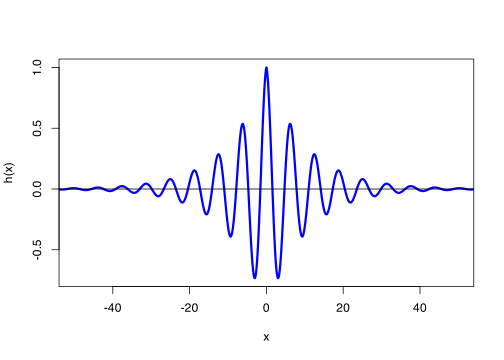
\includegraphics[keepaspectratio]{index_files/mediabag/lectures/L02-mc-uses_files/figure-pdf/h-graph-1.pdf}}

This suggests to me that a mean of 0 and a standard deviation of 20
might work quite well, since this will tend to take values in
\([-40,40]\) or so.

We will use R's function \texttt{dnorm()} for the probability density
function of the normal distribution (which saves us from having to
remember what that is).

\begin{Shaded}
\begin{Highlighting}[]
\NormalTok{n }\OtherTok{\textless{}{-}} \FloatTok{1e6}
\NormalTok{integrand }\OtherTok{\textless{}{-}} \ControlFlowTok{function}\NormalTok{(x) }\FunctionTok{exp}\NormalTok{(}\SpecialCharTok{{-}}\FloatTok{0.1} \SpecialCharTok{*} \FunctionTok{abs}\NormalTok{(x)) }\SpecialCharTok{*} \FunctionTok{cos}\NormalTok{(x)}
\NormalTok{pdf       }\OtherTok{\textless{}{-}} \ControlFlowTok{function}\NormalTok{(x) }\FunctionTok{dnorm}\NormalTok{(x, }\DecValTok{0}\NormalTok{, }\DecValTok{20}\NormalTok{)}
\NormalTok{phi       }\OtherTok{\textless{}{-}} \ControlFlowTok{function}\NormalTok{(x) }\FunctionTok{integrand}\NormalTok{(x) }\SpecialCharTok{/} \FunctionTok{pdf}\NormalTok{(x)}

\NormalTok{samples }\OtherTok{\textless{}{-}} \FunctionTok{rnorm}\NormalTok{(n, }\DecValTok{0}\NormalTok{, }\DecValTok{20}\NormalTok{)}
\FunctionTok{mean}\NormalTok{(}\FunctionTok{phi}\NormalTok{(samples))}
\end{Highlighting}
\end{Shaded}

\begin{verbatim}
[1] 0.2189452
\end{verbatim}

\end{example}

\textbf{Next time:} \emph{We will analyse the accuracy of these Monte
Carlo estimates.}

\textbf{Summary:}

\begin{itemize}
\item
  The indicator \(\Ind_A(x)\) function of a set \(A\) is 1 if
  \(x \in A\) or 0 if \(x \notin A\).
\item
  We can estimate a probability \(\mathbb P(X \in A)\) by using the
  Monte Carlo estimate for \(\Exg\Ind_A(X)\).
\item
  We can estimate an integral \(\int h(x) \, \mathrm{d}x\) by using a
  Monte Carlo estimate with \(\phi(x)\,f(x) = h(x)\).
\end{itemize}

\textbf{Read more:}
\href{https://leeds.primo.exlibrisgroup.com/permalink/44LEE_INST/1fj430b/cdi_askewsholts_vlebooks_9781118728031}{Voss,
\emph{An Introduction to Statistical Computing}}, Section 3.1 and
Subsection 3.2.1.

\chapter{Monte Carlo error I: theory}\label{monte-carlo-error-i-theory}

\[ \]

\section{Estimation error}\label{estimation-error}

Today we are going to analysing the accuracy of Monte Carlo estimation.
But before talking about Monte Carlo estimation specifically, let's
first remind ourselves of some concepts about error in statistical
estimation more generally. We will use the following definitions.

\begin{definition}[]\protect\hypertarget{def-stats}{}\label{def-stats}

Let \(\widehat\theta\) be an estimator of a parameter \(\theta\). Then
we have the following definitions of the estimator \(\widehat\theta\):

\begin{itemize}
\item
  The \textbf{bias} is
  \(\operatorname{bias}\big(\widehat\theta\big) = \mathbb E\big(\widehat\theta - \theta\big)  = \mathbb E\widehat\theta - \theta\).
\item
  The \textbf{mean-square error} is
  \(\operatorname{MSE}\big(\widehat\theta\big) = \mathbb E \big(\widehat\theta - \theta\big)^2\).
\item
  The \textbf{root-mean-square error} is the square-root of the
  mean-square error,
  \[\operatorname{RMSE}\big(\widehat\theta\big) = \sqrt{\operatorname{MSE}(\widehat\theta)} = \sqrt{\mathbb E (\widehat\theta - \theta)^2} . \]
\end{itemize}

\end{definition}

Usually, the main goal of estimation is to get the mean-square error of
an estimate as small as possible. This is because the MSE measures by
what distance we are missing on average. It can be easier to interpret
what the root-mean-square error means, as the RMSE has the same units as
the parameter being measured: if \(\theta\) and \(\widehat{\theta}\) are
in metres, say, then the MSE is in metres-squared, whereas the RMSE
error is in metres again. If you minimise the MSE you also minimise the
RMSE and vice versa.

It's nice to have an ``unbiased'' estimator -- that is, one with bias 0.
This is because bias measures any systematic error in a particular
direction. However, unbiasedness by itself is not enough for an estimate
to be good -- we need low variance too. (Remember the old joke about the
statistician who misses his first shot ten yards to the left, misses his
second shot ten yards to the right, then claims to have ``hit the target
on average.'')

(Remember also that ``bias'' is simply the word statisticians use for
\(\mathbb E(\widehat\theta - \theta)\); we don't mean ``bias'' in the
derogatory way it is sometimes used in political arguments, for
example.)

You probably also remember the relationship between the mean-square
error, the bias, and the variance:

\begin{theorem}[]\protect\hypertarget{thm-MSE-bias}{}\label{thm-MSE-bias}

~
\(\operatorname{MSE}\big(\widehat\theta\big) = \operatorname{bias}\big(\widehat\theta\big)^2 + \operatorname{Var}\big(\widehat\theta\big)\).

\end{theorem}

\begin{proof}
The MSE is \begin{align}
  \operatorname{MSE}\big(\widehat\theta\big) = \Exg\big(\widehat\theta - \theta\big)^2
    &= \Exg \big(\widehat\theta^2 - 2\theta\widehat\theta + \theta\big)^2 \\
    &= \Exg \widehat\theta^2 - 2\theta \Exg \widehat\theta + \theta^2 ,
\end{align} where we have expanded the brackets and bought the
expectation inside (remembering that \(\theta\) is a constant). Since
the variance can be written as
\(\Var(\widehat\theta) = \Exg\widehat\theta^2 - (\Exg \widehat\theta)^2\),
we can use a cunning trick of both subtracting and adding
\((\Exg \widehat\theta)^2\). This gives \begin{align}
\operatorname{MSE}\big(\widehat\theta\big)
  &= \Exg \widehat\theta^2 - \big(\!\Exg \widehat\theta\big)^2 + \big(\!\Exg \widehat\theta\big)^2 - 2\theta \Exg \widehat\theta + \theta^2 \\
  &= \Var\big(\widehat\theta\big) + \big( (\Exg \widehat\theta)^2 - 2\theta \Exg \widehat\theta + \theta^2 \big) \\
  &= \Var\big(\widehat\theta\big) + \big( \! \Exg \widehat\theta - \theta\big)^2 \\
  &= \Var\big(\widehat\theta\big) + \operatorname{bias}(\widehat\theta)^2 .
\end{align} This proves the result.
\end{proof}

Since the bias contributes to the mean-square error, that's another
reason to like estimator with low -- or preferably zero -- bias. But
again, unbiasedness isn't enough by itself; we want low variance too.
(There are some situations where there's a ``bias--variance tradeoff'',
where allowing some bias reduces the variance and so can reduce the MSE.
It turns out that Monte Carlo is not one of these cases, however.)

\section{Error of Monte Carlo estimator:
theory}\label{error-of-monte-carlo-estimator-theory}

In this lecture, we're going to be looking more carefully at the size of
the errors made by the Monte Carlo estimator
\[ \widehat{\theta}_n^{\mathrm{MC}} = \frac{1}{n} \big(\phi(X_1) + \phi(X_2) + \cdots + \phi(X_n) \big) = \frac{1}{n} \sum_{i=1}^n \phi(X_i) . \]

Our main result is the following.

\begin{theorem}[]\protect\hypertarget{thm-MCerr}{}\label{thm-MCerr}

Let \(X\) be a random variable, \(\phi\) a function, and
\(\theta = \Exg\phi(X)\). Let
\[ \widehat{\theta}_n^{\mathrm{MC}} = \frac{1}{n} \sum_{i=1}^n \phi(X_i) \]
be the Monte Carlo estimator of \(\theta\). Then:

\begin{enumerate}
\def\labelenumi{\arabic{enumi}.}
\item
  \(\widehat{\theta}_n^{\mathrm{MC}}\) is unbiased, in that
  \(\operatorname{bias}\big(\widehat{\theta}_n^{\mathrm{MC}}\big) = 0\).
\item
  The variance of of \(\widehat{\theta}_n^{\mathrm{MC}}\) is
  \({\displaystyle \operatorname{Var}\big(\widehat{\theta}_n^{\mathrm{MC}}\big) = \frac{1}{n} \operatorname{Var}\big(\phi(X)\big)}\).
\item
  The mean-square error of \(\widehat{\theta}_n^{\mathrm{MC}}\) is
  \({\displaystyle \operatorname{MSE}\big(\widehat{\theta}_n^{\mathrm{MC}}\big) = \frac{1}{n} \operatorname{Var}\big(\phi(X)\big)}\).
\item
  The root-mean-square error of \(\widehat{\theta}_n^{\mathrm{MC}}\) is
  \[{\displaystyle \operatorname{RMSE}\big(\widehat{\theta}_n^{\mathrm{MC}}\big) = \sqrt{\frac{1}{n} \operatorname{Var}\big(\phi(X)\big)} = \frac{1}{\sqrt{n}} \, \operatorname{sd}\big(\phi(X)\big)}. \]
\end{enumerate}

\end{theorem}

Before we get to the proof, let's recap some relevant probability.

Let \(Y_1, Y_2, \dots\) be IID random variables with common expectation
\(\mathbb EY_1 = \mu\) and common variance
\(\operatorname{Var}(Y_1) = \sigma^2\). Consider the mean of the first
\(n\) random variables,
\[ \overline{Y}_n = \frac{1}{n} \sum_{i=1}^n Y_i . \] Then the
expectation of \(\overline{Y}_n\) is
\[ \mathbb E \overline{Y}_n = \mathbb E\left(\frac{1}{n}\sum_{i=1}^n Y_i\right) = \frac{1}{n} 
\sum_{i=1}^n \mathbb{E}Y_i = \frac{1}{n}\,n\,\mu = \mu . \] The variance
of \(\overline{Y}_n\) is
\[ \operatorname{Var}\big(  \overline{Y}_n \big)= \operatorname{Var} \left(\frac{1}{n}\sum_{i=1}^n Y_i\right) = \bigg(\frac{1}{n}\bigg)^2 
\sum_{i=1}^n \operatorname{Var}(Y_i) = \frac{1}{n^2}\,n\,\sigma^2 = \frac{\sigma^2}{n} , \]
where, for this one, we used the independence of the random variables.

\begin{proof}
Apply the probability facts from above with \(Y = \phi(X)\). This gives:

\begin{enumerate}
\def\labelenumi{\arabic{enumi}.}
\item
  \(\Ex \widehat{\theta}_n^{\mathrm{MC}} = \Ex \overline Y_n = \Ex Y = \Exg \phi(X)\),
  so
  \(\operatorname{bias}(\widehat{\theta}_n^{\mathrm{MC}}) = \Exg \phi(X) - \Exg \phi(X) = 0\).
\item
  \({\displaystyle \operatorname{Var}\big(\widehat{\theta}_n^{\mathrm{MC}}\big) = \operatorname{Var}\big(\overline Y_n\big) = \frac{1}{n} \operatorname{Var}(Y) = \frac{1}{n} \operatorname{Var}\big(\phi(X)\big)}\).
\item
  Using Theorem~\ref{thm-MSE-bias},
  \[\operatorname{MSE}(\widehat{\theta}_n^{\mathrm{MC}}) = \operatorname{bias}(\widehat{\theta}_n^{\mathrm{MC}})^2 + \operatorname{Var}(\widehat{\theta}_n^{\mathrm{MC}}) = 0^2 + \frac{1}{n} \operatorname{Var}\big(\phi(X)\big) = \frac{1}{n} \operatorname{Var}\big(\phi(X)\big) . \]
\item
  Take the square root of part 3.
\end{enumerate}

\end{proof}

Let's think about MSE \(\frac{1}{n} \Var(\phi(X))\). The variance terms
is some fixed fact about the random variable \(X\) and the function
\(\phi\). So as \(n\) gets bigger, \(\frac{1}{n}\) gets smaller, so the
MSE gets smaller, and the estimator gets more accurate. This goes back
to what we said when we introduced the Monte Carlo estimator: we get a
more accurate estimate by increasing \(n\). More specifically, the MSE
scales like \(1/n\), or -- perhaps a more useful result -- the RMSE
scales like \(1/\sqrt{n}\). We'll come back to this in the next lecture.

\section{Error of Monte Carlo estimator:
practice}\label{error-of-monte-carlo-estimator-practice}

So when we form a Monte Carlo estimate \(\hat\theta_n^{\text{MC}}\), we
now know it will be unbiased. We'd also like to know it's mean-square
and/or root-mean-square error too.

There's a problem here, though. The reason we are doing Monte Carlo
estimation in the first place is that we \emph{couldn't} calculate
\(\Exg \phi(X)\). So it seems very unlikely we'll be able to calculate
the variance \(\operatorname{Var}(\phi(X))\) either. So how will be able
to assess the mean-square (or root-mean-square) error of our Monte Carlo
estimator?

Well, we can't know it exactly. But we \emph{can} estimate the variance
from the samples we are already using: by taking the sample variance of
the samples \(\phi(x_i)\). That is, we can estimate the variance of the
Monte Carlo estimator by the sample variance
\[ S^2 = \frac{1}{n-1} \sum_{i=1}^n \big(\phi(X_i) - \widehat{\theta}_n^{\mathrm{MC}} \big)^2 . \]
Then we can similarly estimate the mean-square and root-mean-square
errors by
\[ \text{MSE} \approx \frac{1}{n}S^2 \qquad \text{and} \qquad \text{RMSE} \approx \sqrt{\frac{1}{n} S^2} = \frac{1}{\sqrt{n}}\,S  \]
respectively.

\begin{example}[]\protect\hypertarget{exm-MCexp2}{}\label{exm-MCexp2}

Let's go back to the very first example in the module,
Example~\ref{exm-MCexp}, where we were trying to find the expectation of
an \(\operatorname{Exp}(2)\) random variable. We used this R code:

\begin{Shaded}
\begin{Highlighting}[]
\NormalTok{n }\OtherTok{\textless{}{-}} \FloatTok{1e6}
\NormalTok{samples }\OtherTok{\textless{}{-}} \FunctionTok{rexp}\NormalTok{(n, }\DecValTok{2}\NormalTok{)}
\NormalTok{MCest }\OtherTok{\textless{}{-}} \FunctionTok{mean}\NormalTok{(samples)}
\NormalTok{MCest}
\end{Highlighting}
\end{Shaded}

\begin{verbatim}
[1] 0.5006352
\end{verbatim}

(Because Monte Carlo estimation is random, this won't be the
\emph{exact} same estimate we had before, of course.)

So if we want to investigate the error, we can use the sample variance
of these samples. We will use the sample variance function
\texttt{var()} to calculate the sample variance. In this simple case,
the function is \(\phi(x) = x\), so we need only use the variance of the
samples themselves.

\begin{Shaded}
\begin{Highlighting}[]
\NormalTok{var\_est }\OtherTok{\textless{}{-}} \FunctionTok{var}\NormalTok{(samples)}
\NormalTok{MSEest  }\OtherTok{\textless{}{-}}\NormalTok{ var\_est }\SpecialCharTok{/}\NormalTok{ n}
\NormalTok{RMSEest }\OtherTok{\textless{}{-}} \FunctionTok{sqrt}\NormalTok{(MSEest)}
\FunctionTok{c}\NormalTok{(var\_est, MSEest, RMSEest)}
\end{Highlighting}
\end{Shaded}

\begin{verbatim}
[1] 2.503570e-01 2.503570e-07 5.003569e-04
\end{verbatim}

The first number is \texttt{var\_est} \(= 0.2504\), the sample variance
of our \(\phi(x_i)\)s:\\
\[ s^2 = \frac{1}{n-1} \sum_{i=1}^n \big(\phi(x_i) - \widehat{\theta}_n^{\mathrm{MC}}\big)^2 . \]
This should be a good estimate of the true variance
\(\operatorname{Var}(\phi(X))\). (In fact, in this simple case, we know
that \(\operatorname{Var}(X) = \frac{1}{2^2} = 0.25\), so we know that
the estimate is good.) In calculating this in the code, we used R's
\texttt{var()} function, which calculates the sample variance of some
values.

The second number is \texttt{MSEest}
\(= \ensuremath{2.504\times 10^{-7}}\), our estimate of the mean-square
error. Since
\(\operatorname{MSE}(\widehat{\theta}_n^{\mathrm{MC}}) = \frac{1}{n} \operatorname{Var}(\phi(X))\),
then \(\frac{1}{n} S^2\) should be a good estimate of the MSE.

The third number is \texttt{RMSEest} \(= \ensuremath{5\times 10^{-4}}\)
our estimate of the root-mean square error, which is simply the
square-root of our estimate of the mean-square error.

\end{example}

\begin{example}[]\protect\hypertarget{exm-MCprob2}{}\label{exm-MCprob2}

In Example~\ref{exm-MCprob}, we were estimating \(\mathbb P(Z > 2)\),
where \(Z\) is a standard normal.

Our code was

\begin{Shaded}
\begin{Highlighting}[]
\NormalTok{n }\OtherTok{\textless{}{-}} \FloatTok{1e6}
\NormalTok{samples }\OtherTok{\textless{}{-}} \FunctionTok{rnorm}\NormalTok{(n)}
\NormalTok{MCest }\OtherTok{\textless{}{-}} \FunctionTok{mean}\NormalTok{(samples }\SpecialCharTok{\textgreater{}} \DecValTok{2}\NormalTok{)}
\NormalTok{MCest}
\end{Highlighting}
\end{Shaded}

\begin{verbatim}
[1] 0.022458
\end{verbatim}

So our root-mean-square error can be approximated as

\begin{Shaded}
\begin{Highlighting}[]
\NormalTok{MSEest }\OtherTok{\textless{}{-}} \FunctionTok{var}\NormalTok{(samples }\SpecialCharTok{\textgreater{}} \DecValTok{2}\NormalTok{) }\SpecialCharTok{/}\NormalTok{ n}
\FunctionTok{sqrt}\NormalTok{(MSEest)}
\end{Highlighting}
\end{Shaded}

\begin{verbatim}
[1] 0.0001481677
\end{verbatim}

since \texttt{samples\ \textgreater{}\ 2} is the indicator function of
whether \(X_i > 2\) or not.

\end{example}

\textbf{Next time:} \emph{We'll continue analysing Monte Carlo error,
looking at confidence intervals and assessing how many samples to
take..}

\textbf{Summary:}

\begin{itemize}
\item
  The Monte Carlo estimator is unbiased.
\item
  The Monte Carlo estimator has mean-square error \(\Var(\phi(X))/n\),
  so the root-mean-square error scales like \(1/\sqrt{n}\).
\item
  The mean-square error can be estimated by \(S^2 / n\), where \(S^2\)
  is the sample variance of the \(\phi(X_i)\).
\end{itemize}

\textbf{Read more:}
\href{https://leeds.primo.exlibrisgroup.com/permalink/44LEE_INST/1fj430b/cdi_askewsholts_vlebooks_9781118728031}{Voss,
\emph{An Introduction to Statistical Computing}}, Subsection 3.2.2.

\chapter{Monte Carlo error II:
practice}\label{monte-carlo-error-ii-practice}

\[ \]

\section{Recap}\label{recap}

Let's recap where we've got to. We know that the Monte Carlo estimator
for \(\theta = \Exg \phi(X)\) is
\[ \widehat{\theta}_n^{\mathrm{MC}} = \frac{1}{n} \sum_{i=1}^n \phi(X_i) .\]
Last time, we saw that the Monte Carlo estimator is unbiased, and that
its mean-square and root-mean-square errors are
\[ \operatorname{MSE}\big(\widehat{\theta}_n^{\mathrm{MC}}\big) = \frac{1}{n} \operatorname{Var}\big(\phi(X)\big) \qquad \operatorname{RMSE}\big(\widehat{\theta}_n^{\mathrm{MC}}\big) = \sqrt{\frac{1}{n} \operatorname{Var}\big(\phi(X)\big)} . \]
We saw that these themselves can be estimated as \(S^2/n\) and
\(S/\sqrt{n}\) respectively, where \(S^2\) is the sample variance of the
\(\phi(X_i)\)s.

\section{Confidence intervals}\label{confidence-intervals}

So far, we have described our error tolerance in terms of the MSE or
RMSE. But we could have talked about ``confidence intervals'' or
``margins of error'' instead. This might be easier to understand for
non-mathematicians, for whom ``root-mean-square error'' doesn't really
mean anything.

Here, we will want to appeal to the central limit theorem approximation.
A bit more probability revision: Let \(Y_1, Y_2, \dots\) be IID again,
with expectation \(\mu\) and variance \(\sigma^2\). Write
\(\overline Y_n\) for the mean. We've already reminded ourselves of the
law of large numbers, which says that \(\overline Y_n \to \mu\) as
\(n \to infty\). Then in the last lecture we saw that
\(\mathbb E \overline Y_n = \mu\) and
\(\Var(\overline{Y}_n) = \sigma^2/n\). The \textbf{central limit
theorem} says that the distribution of \(\overline Y_n\) is
approximately normally distributed with those parameters, so
\(\overline Y_n \approx \operatorname{N}(\mu, \sigma^2/n)\) when \(n\)
is large. (This is an informal statement of the central limit theorem:
you probably know some more formal ways to more precisely state it, but
this will do for us.)

Recall that, in the normal distribution
\(\operatorname{N}(\mu, \sigma^2)\), we expect to be within \(1.96\)
standard deviations of the mean with 95\% probability. More generally,
the interval
\([\mu - q_{1-\alpha/2}\sigma, \mu + q_{1-\alpha/2}\sigma]\), where
\(q_{1-\alpha/2}\) is the \((1- \frac{\alpha}{2})\)-quantile of the
normal distribution, contains the true value with probability
approximately \(1 - \alpha\).

We can form an approximate confidence interval for a Monte Carlo
estimate using this idea. We have our Monte Carlo estimator
\(\widehat{\theta}_n^\mathrm{MC}\) as our estimator of the \(\mu\)
parameter, and our estimator of the root-mean-square error
\(S/\sqrt{n}\) as our estimator of the \(\sigma\) parameter. So our
confidence interval is estimated as
\[\bigg[ \widehat{\theta}_n^\mathrm{MC} - q_{1-\alpha/2}\,\frac{S}{\sqrt{n}}, \ \widehat{\theta}_n^\mathrm{MC} + q_{1-\alpha/2}\,\frac{S}{\sqrt{n}} \bigg] . \]

\begin{example}[]\protect\hypertarget{exm-MCprob3}{}\label{exm-MCprob3}

We continue the example of Example~\ref{exm-MCprob} and
Example~\ref{exm-MCprob2}, where we were estimating \(\mathbb P(Z > 2)\)
for \(Z\) a standard normal.

\begin{Shaded}
\begin{Highlighting}[]
\NormalTok{n }\OtherTok{\textless{}{-}} \FloatTok{1e6}
\NormalTok{samples }\OtherTok{\textless{}{-}} \FunctionTok{rnorm}\NormalTok{(n)}
\NormalTok{MCest   }\OtherTok{\textless{}{-}} \FunctionTok{mean}\NormalTok{(samples }\SpecialCharTok{\textgreater{}} \DecValTok{2}\NormalTok{)}
\NormalTok{RMSEest }\OtherTok{\textless{}{-}} \FunctionTok{sqrt}\NormalTok{(}\FunctionTok{var}\NormalTok{(samples }\SpecialCharTok{\textgreater{}} \DecValTok{2}\NormalTok{) }\SpecialCharTok{/}\NormalTok{ n)}
\NormalTok{MCest}
\end{Highlighting}
\end{Shaded}

\begin{verbatim}
[1] 0.023177
\end{verbatim}

Our confidence interval is estimates as follows

\begin{Shaded}
\begin{Highlighting}[]
\NormalTok{alpha }\OtherTok{\textless{}{-}} \FloatTok{0.05}
\NormalTok{quant }\OtherTok{\textless{}{-}} \FunctionTok{qnorm}\NormalTok{(}\DecValTok{1} \SpecialCharTok{{-}}\NormalTok{ alpha }\SpecialCharTok{/} \DecValTok{2}\NormalTok{)}
\FunctionTok{c}\NormalTok{(MCest }\SpecialCharTok{{-}}\NormalTok{ quant }\SpecialCharTok{*}\NormalTok{ RMSEest, MCest }\SpecialCharTok{+}\NormalTok{ quant }\SpecialCharTok{*}\NormalTok{ RMSEest)}
\end{Highlighting}
\end{Shaded}

\begin{verbatim}
[1] 0.02288209 0.02347191
\end{verbatim}

\end{example}

\section{How many samples do I need?}\label{how-many-samples-do-i-need}

In our examples we've picked the number of samples \(n\) for our
estimator, then approximated the error based on that. But we could do
things the other way around -- fix an error tolerance that we're willing
to deal with, then work out what sample size we need to achieve it.

We know that the root-mean-square error is
\[ \operatorname{RMSE}\big(\widehat{\theta}_n^{\mathrm{MC}}\big) = \sqrt{\frac{1}{n} \operatorname{Var}\big(\phi(X)\big)} \]
So if we want to get the RMSE down to \(\epsilon\), say, then this shows
that we need
\[ \epsilon = \sqrt{\frac{1}{n} \operatorname{Var}\big(\phi(X)\big)} .\]
Squaring both sides, multiplying both sides by \(n\), and dividing both
sides by \(\epsilon^2\) gives
\[ n = \frac{1}{\epsilon^2} \Var\big(\phi(X)\big) . \]

So this tells us how many samples \(n\) we need. Except we still have a
problem here, though. We (usually) don't know \(\Var(\phi(X))\). But we
can't even \emph{estimate} \(\Var(\phi(X))\) until we've already taken
the samples. So it seems we're stuck.

But we can use this idea with a three-step process:

\begin{enumerate}
\def\labelenumi{\arabic{enumi}.}
\item
  Run an initial ``pilot'' Monte Carlo algorithm with a small number of
  samples \(n\). Use the results of the ``pilot'' to estimate the
  variance \(S^2 \approx \Var(\phi(X))\). We want \(n\) small enough
  that this runs very quickly, but big enough that we get a reasonably
  OK estimate of the variance.
\item
  Pick a desired RMSE accuracy \(\epsilon\). We now know that we require
  roughly \(N = S^2 / \epsilon^2\) samples to get our desired accuracy.
\item
  Run the ``real'' Monte Carlo algorithm with this big number of samples
  \(N\). We will put up with this being quite slow, because we know
  we're definitely going to get the error tolerance we need.
\end{enumerate}

(We could potentially use further steps, where we now check the variance
with the ``real'' big-\(N\) samples, and, if we learn we had
underestimated in Step 1, take even more samples to correct for this.)

\begin{example}[]\protect\hypertarget{exm-MC22}{}\label{exm-MC22}

Let's try this with Example~\ref{exm-MC2} from before. We were trying to
estimate \(\mathbb{E}(\sin X)\), where
\(X \sim \operatorname{N}(1, 2^2)\).

We'll start with just \(n = 1000\) samples, for our pilot study.

\begin{Shaded}
\begin{Highlighting}[]
\NormalTok{n\_pilot }\OtherTok{\textless{}{-}} \DecValTok{1000}
\NormalTok{samples }\OtherTok{\textless{}{-}} \FunctionTok{rnorm}\NormalTok{(n\_pilot, }\DecValTok{1}\NormalTok{, }\DecValTok{2}\NormalTok{)}
\NormalTok{var\_est }\OtherTok{\textless{}{-}} \FunctionTok{var}\NormalTok{(}\FunctionTok{sin}\NormalTok{(samples))}
\NormalTok{var\_est}
\end{Highlighting}
\end{Shaded}

\begin{verbatim}
[1] 0.4905153
\end{verbatim}

This was very quick! We won't have got a super-accurate estimate of
\(\mathbb E\phi(X)\), but we have a reasonable idea of roughly what
\(\operatorname{Var}(\phi(X))\) is. This will allow us to pick out
``real'' sample size in order to get a root-mean-square error of
\(10^{-4}\).

\begin{Shaded}
\begin{Highlighting}[]
\NormalTok{epsilon }\OtherTok{\textless{}{-}} \FloatTok{1e{-}4}
\NormalTok{n\_real  }\OtherTok{\textless{}{-}} \FunctionTok{round}\NormalTok{(var\_est }\SpecialCharTok{/}\NormalTok{ epsilon}\SpecialCharTok{\^{}}\DecValTok{2}\NormalTok{)}
\NormalTok{n\_real}
\end{Highlighting}
\end{Shaded}

\begin{verbatim}
[1] 49051535
\end{verbatim}

This tells us that we will need about 50 million samples! This is a lot,
but now we know we're going to get the accuracy we want, so it's worth
it. (In this particular case, 50 million samples will only take a few
second on a modern computer. But generally, once we know our code works
and we know how many samples we will need for the desired accuracy, this
is the sort of thing that we could leave running overnight or whatever.)

\begin{Shaded}
\begin{Highlighting}[]
\NormalTok{samples }\OtherTok{\textless{}{-}} \FunctionTok{rnorm}\NormalTok{(n\_real, }\DecValTok{1}\NormalTok{, }\DecValTok{2}\NormalTok{)}
\NormalTok{MCest }\OtherTok{\textless{}{-}} \FunctionTok{mean}\NormalTok{(}\FunctionTok{sin}\NormalTok{(samples))}
\NormalTok{MCest}
\end{Highlighting}
\end{Shaded}

\begin{verbatim}
[1] 0.1139149
\end{verbatim}

\begin{Shaded}
\begin{Highlighting}[]
\NormalTok{RMSEest }\OtherTok{\textless{}{-}} \FunctionTok{sqrt}\NormalTok{(}\FunctionTok{var}\NormalTok{(}\FunctionTok{sin}\NormalTok{(samples)) }\SpecialCharTok{/}\NormalTok{ n\_real)}
\NormalTok{RMSEest}
\end{Highlighting}
\end{Shaded}

\begin{verbatim}
[1] 9.964886e-05
\end{verbatim}

This second step was quite slow (depending on the speed of the computer
being used -- it was only about 5 seconds on my pretty-new laptop, but
slower on my ancient work desktop). But we see that we have indeed got
our Monte Carlo estimate to (near enough) the desired accuracy.

\end{example}

Generally, if we want a more accurate Monte Carlo estimator, we can just
take more samples. But the equation
\[ n = \frac{1}{\epsilon^2} \Var\big(\phi(X)\big) \] is actually quite
bad news. To get an RMSE of \(\epsilon\) we need order \(1/\epsilon^2\)
samples. That's not good. Think of it like this: to \emph{double} the
accuracy we need to \emph{quadruple} the number of samples. Even worse:
to get ``one more decimal place of accuracy'' means dividing
\(\epsilon\) by ten; but that means multiplying the number of samples by
one hundred!

More samples take more time, and cost more energy and money. Wouldn't it
be nice to have some better ways of increasing the accuracy of a Monte
Carlo estimate besides just taking more and more samples?

\textbf{Next time:} \emph{We begin our study of clever ``variance
reduction'' methods for Monte Carlo estimation.}

\textbf{Summary:}

\begin{itemize}
\item
  We can approximate confidence intervals for a Monte Carlo estimate by
  using a normal approximation.
\item
  To get the root-mean-square error below \(\epsilon\) we need
  \(n = \Var(\phi(X))/\epsilon^2\) samples.
\item
  We can use a two-step process, where a small ``pilot'' Monte Carlo
  estimation allows us to work out how many samples we will need for the
  big ``real'' estimation.
\end{itemize}

\textbf{Read more:}
\href{https://leeds.primo.exlibrisgroup.com/permalink/44LEE_INST/1fj430b/cdi_askewsholts_vlebooks_9781118728031}{Voss,
\emph{An Introduction to Statistical Computing}}, Subsections
3.2.2--3.2.4.

\chapter{Control variate}\label{control-variate}

\[ \]

\section{Variance reduction}\label{variance-reduction}

Let's recap where we've got to. The Monte Carlo estimator of
\(\theta = \Exg \phi(X)\) is
\[ \widehat{\theta}_n^{\mathrm{MC}} = \frac{1}{n} \sum_{i=1}^n \phi(X_i), \]
where \(X_1, X_2, \dots, X_n\) are IID random samples from \(X\). The
mean-square error of this estimator is
\[{\displaystyle \operatorname{MSE}\big(\widehat{\theta}_n^{\mathrm{MC}}\big) = \frac{1}{n} \operatorname{Var}\big(\phi(X)\big)} . \]
If we want a more accurate estimate, we can just take more samples
\(n\). But the problem is that the root-mean-square error scales like
\(1/\sqrt{n}\). To double the accuracy, we need four times as many
samples; for one more decimal place of accuracy, we need one hundred
times as many samples.

Are there other ways we could reduce the error of Monte Carlo
estimation, so we need fewer samples? That is, can we use some
mathematical ingenuity to adapt the Monte Carlo estimate to one with a
smaller error?

Well, the mean-square error is the variance divided by \(n\). So if we
can't (or don't want to) increase \(n\), perhaps we can \emph{decrease}
the \emph{variance} instead? Strategies to do this are called
\textbf{variance reduction strategies}. In this module, we will look at
three variance reduction strategies:

\begin{itemize}
\item
  \textbf{Control variate:} We can ``anchor'' our estimate of
  \(\Exg \phi(X)\) to a similar but easier-to-calculate value
  \(\Exg \psi(X)\). (This lecture)
\item
  \textbf{Antithetic variables:} Instead of using independent samples,
  we could use correlated samples. If the correlation is negative this
  can improve our estimate. (Lectures 6 and 7)
\item
  \textbf{Importance sampling:} Instead of sampling from \(X\), sample
  from some other more suitable distribution instead, then adjust the
  answer we get. (Lectures 8 and 9)
\end{itemize}

\section{Control variate estimation}\label{control-variate-estimation}

In Monday's lecture, I polled the class on this question: \emph{Estimate
the average time it takes to fly from London to New York.}

\begin{itemize}
\item
  The actual answer is: 8 hours.
\item
  The mean guess was: 9 hours and 38 minutes (98 minutes too much)
\item
  The root-mean-square error for the guesses was: 158 minutes
\end{itemize}

After you'd guessed, I gave the following hint: \emph{Hint: The average
time it takes to fly from London to Washington D.C. is 8 hours and 15
minutes.} After the hint:

\begin{itemize}
\item
  The mean guess was: 8 hours and 50 minutes (50 minutes too much)
\item
  The root-mean-square error for the guesses was: 72 minutes
\end{itemize}

So after the hint, the error of the class was reduced by 55\%.

(Incidentally, you were about 30\% at guessing this than last year's
students\ldots)

Why did the hint help? We were trying to estimate
\(\theta^{\mathrm{NY}}\), the distance to New York. But that's a big
number, and the first estimates had a big error (over an hour, on
average). After the hint, I expect most people thought something like
this: ``The answer \(\theta^{\mathrm{NY}}\) is going to be similar to
the \(\theta^{\mathrm{DC}} =\) 8:15 to Washington D.C., but New York
isn't quite as far, so I should decrease the number a bit, but not too
much.''

To be more mathematical, we could write
\[\theta^{\mathrm{NY}} = \theta^{\mathrm{NY}} + \big(\theta^{\mathrm{DC}} - \theta^{\mathrm{DC}}\big) =  \underbrace{\theta^{\mathrm{DC}}\vphantom{\big)}}_{\text{known}} + \underbrace{\big(\theta^{\mathrm{NY}} - \theta^{\mathrm{DC}}\big)}_{\text{small}} . \]
In that equation, the first term, \(\theta^{\mathrm{DC}} =\) 8:15 was
completely known, so had error 0, while the second term
\(\theta^{\mathrm{NY}} - \theta^{\mathrm{DC}}\) (actually minus 15
minutes) was a small number, so only had a small error.

This idea of improving an estimate by ``anchoring'' it to some known
value is called \textbf{controlled estimation}. It is a very useful idea
in statistics (and in life!).

We can apply this idea to Monte Carlo estimation too. Suppose we are
trying to estimate \(\theta = \Exg \phi(X)\). We could look for a
function \(\psi\) that is similar to \(\phi\) (at least for the values
of \(x\) that have high probability for the random variable \(X\)), but
where we know for certain what \(\Exg \psi(X)\) is. Then we can write
\[ \theta = \Exg \phi(X) = \Exg \big(\phi(X) - \psi(X) + \psi(X)\big) = \underbrace{\Exg\big(\phi(X) - \psi(X)\big)}_{\text{estimate this with Monte Carlo}} + \underbrace{\Exg \psi(X)\vphantom{\big)}}_{\text{known}} . \]

Here, \(\psi(X)\) is known as the \textbf{control variate}.

\begin{definition}[]\protect\hypertarget{def-MCest}{}\label{def-MCest}

Let \(X\) be a random variable, \(\phi\) a function, and write
\(\theta = \Exg\phi(X)\). Let \(\psi\) be a function such that
\(\eta = \Exg\psi(X)\) is known. Suppose that \(X_1, X_2, \dots, X_n\)
are a random sample from \(X\). Then the \textbf{control variate Monte
Carlo estimate} \(\widehat\theta_n^{\mathrm{CV}}\) of \(\theta\) is
\[ \widehat{\theta}_n^{\mathrm{CV}} = \frac{1}{n} \sum_{i=1}^n \big(\phi(X_i) - \psi(X_i)\big) + \eta . \]

\end{definition}

\begin{example}[]\protect\hypertarget{exm-control}{}\label{exm-control}

Let's try to estimate \(\Ex \cos(X)\), where
\(X \sim \operatorname{N}(0,1)\) is a standard normal distribution.

We could do this the ``usual'' Monte Carlo way.

\begin{Shaded}
\begin{Highlighting}[]
\NormalTok{n }\OtherTok{\textless{}{-}} \FloatTok{1e6}
\NormalTok{phi }\OtherTok{\textless{}{-}} \ControlFlowTok{function}\NormalTok{(x) }\FunctionTok{cos}\NormalTok{(x)}
\NormalTok{samples }\OtherTok{\textless{}{-}} \FunctionTok{rnorm}\NormalTok{(n)}
\NormalTok{MCest }\OtherTok{\textless{}{-}} \FunctionTok{mean}\NormalTok{(}\FunctionTok{phi}\NormalTok{(samples))}
\NormalTok{MCest}
\end{Highlighting}
\end{Shaded}

\begin{verbatim}
[1] 0.6067224
\end{verbatim}

But we could see if we can do better with a control variate. But what
should we pick for the control function \(\psi\)? We want something
that's similar to \(\phi(x) = \cos(x)\), but where we can actually
calculate the expectation.

Here's a suggestion. If we remember our
\href{https://en.wikipedia.org/wiki/Taylor_series}{Taylor series}, we
know that, for \(x\) near \(0\),
\[ \cos x \approx 1 - \frac{x^2}{2!} + \frac{x^4}{4!} - \frac{x^6}{6!} + \cdots . \]
So how about taking the first two nonzero terms in the Taylor series
\[ \psi(x) = 1 - \frac{x^2}{2} . \] That is quite close to \(\cos x\),
at least for the values of \(x\) near 0 that
\(X \sim \operatorname{N}(0,1)\) is most likely to take.

\begin{Shaded}
\begin{Highlighting}[]
\FunctionTok{curve}\NormalTok{(}
  \FunctionTok{cos}\NormalTok{(x), }\AttributeTok{from =} \SpecialCharTok{{-}}\FloatTok{4.5}\NormalTok{, }\AttributeTok{to =} \FloatTok{4.5}\NormalTok{,}
  \AttributeTok{col =} \StringTok{"blue"}\NormalTok{, }\AttributeTok{lwd =} \DecValTok{3}\NormalTok{,}
  \AttributeTok{xlab =} \StringTok{"x"}\NormalTok{, }\AttributeTok{ylab =} \StringTok{""}\NormalTok{, }\AttributeTok{xlim =} \FunctionTok{c}\NormalTok{(}\SpecialCharTok{{-}}\DecValTok{4}\NormalTok{,}\DecValTok{4}\NormalTok{), }\AttributeTok{ylim =} \FunctionTok{c}\NormalTok{(}\SpecialCharTok{{-}}\FloatTok{1.2}\NormalTok{,}\FloatTok{1.2}\NormalTok{)}
\NormalTok{)}
\FunctionTok{curve}\NormalTok{(}\DecValTok{1} \SpecialCharTok{{-}}\NormalTok{ x}\SpecialCharTok{\^{}}\DecValTok{2} \SpecialCharTok{/} \DecValTok{2}\NormalTok{, }\AttributeTok{add =} \ConstantTok{TRUE}\NormalTok{, }\AttributeTok{col =} \StringTok{"red"}\NormalTok{, }\AttributeTok{lwd =} \DecValTok{2}\NormalTok{)}
\FunctionTok{legend}\NormalTok{(}
  \StringTok{"topright"}\NormalTok{, }\FunctionTok{c}\NormalTok{(}\StringTok{"cos x"}\NormalTok{, }\FunctionTok{expression}\NormalTok{(}\DecValTok{1} \SpecialCharTok{{-}}\NormalTok{ x}\SpecialCharTok{\^{}}\DecValTok{2} \SpecialCharTok{/} \DecValTok{2}\NormalTok{)),}
  \AttributeTok{lwd =} \FunctionTok{c}\NormalTok{(}\DecValTok{3}\NormalTok{, }\DecValTok{2}\NormalTok{), }\AttributeTok{col =} \FunctionTok{c}\NormalTok{(}\StringTok{"blue"}\NormalTok{, }\StringTok{"red"}\NormalTok{)}
\NormalTok{)}
\end{Highlighting}
\end{Shaded}

\pandocbounded{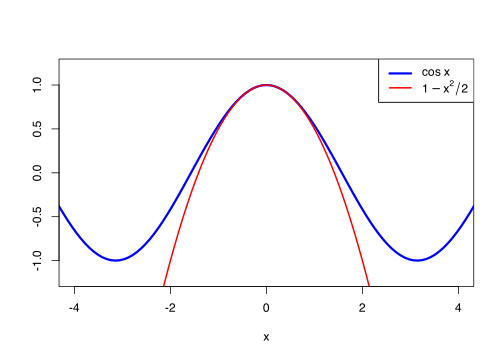
\includegraphics[keepaspectratio]{index_files/mediabag/lectures/L05-cv_files/figure-pdf/taylor-1.pdf}}

Not only that, but we know that for
\(Y \sim \operatorname{N}(\mu, \sigma^2)\) we have
\(\Ex Y^2 = \mu^2 + \sigma^2\). So
\[ \Exg \psi(X) = \Exg \left(1 - \frac{X^2}{2} \right) = 1 - \frac{\Ex X^2}{2} = 1 - \frac{0^2 + 1}{2} = \frac12 . \]

So our control variate estimate is:

\begin{Shaded}
\begin{Highlighting}[]
\NormalTok{psi }\OtherTok{\textless{}{-}} \ControlFlowTok{function}\NormalTok{(x) }\DecValTok{1} \SpecialCharTok{{-}}\NormalTok{ x}\SpecialCharTok{\^{}}\DecValTok{2} \SpecialCharTok{/} \DecValTok{2}
\NormalTok{CVest }\OtherTok{\textless{}{-}} \FunctionTok{mean}\NormalTok{(}\FunctionTok{phi}\NormalTok{(samples) }\SpecialCharTok{{-}} \FunctionTok{psi}\NormalTok{(samples)) }\SpecialCharTok{+} \DecValTok{1}\SpecialCharTok{/}\DecValTok{2}
\NormalTok{CVest}
\end{Highlighting}
\end{Shaded}

\begin{verbatim}
[1] 0.6060243
\end{verbatim}

\end{example}

\section{Error of control variate
estimate}\label{error-of-control-variate-estimate}

What is the error in a control variate estimate?

\begin{theorem}[]\protect\hypertarget{thm-CVerr}{}\label{thm-CVerr}

Let \(X\) be a random variable, \(\phi\) a function, and
\(\theta = \Exg\phi(X)\). Let \(\psi\) be a function such that
\(\eta \Exg\psi(X)\) is known. Let
\[ \widehat{\theta}_n^{\mathrm{CV}} = \frac{1}{n} \sum_{i=1}^n \big(\phi(X_i) - \psi(X_i)\big) + \eta\]
be the control variate Monte Carlo estimator of \(\theta\). Then:

\begin{enumerate}
\def\labelenumi{\arabic{enumi}.}
\item
  \(\widehat{\theta}_n^{\mathrm{CV}}\) is unbiased, in that
  \(\operatorname{bias}\big(\widehat{\theta}_n^{\mathrm{CV}}\big) = 0\).
\item
  The variance of of \(\widehat{\theta}_n^{\mathrm{CV}}\) is
  \({\displaystyle \operatorname{Var}\big(\widehat{\theta}_n^{\mathrm{CV}}\big) = \frac{1}{n} \operatorname{Var}\big(\phi(X) - \psi(X)\big)}\).
\item
  The mean-square error of \(\widehat{\theta}_n^{\mathrm{CV}}\) is
  \({\displaystyle \operatorname{MSE}\big(\widehat{\theta}_n^{\mathrm{CV}}\big) = \frac{1}{n} \operatorname{Var}\big(\phi(X) - \psi(X)\big)}\).
\item
  The root-mean-square error of \(\widehat{\theta}_n^{\mathrm{CV}}\) is
  \({\displaystyle \operatorname{RMSE}\big(\widehat{\theta}_n^{\mathrm{CV}}\big) = \frac{1}{\sqrt{n}} \sqrt{\operatorname{Var}\big(\phi(X) - \psi(X)\big)}}\).
\end{enumerate}

\end{theorem}

\begin{proof}
This is very similar to Theorem~\ref{thm-MCerr}, so we'll just sketch
the important differences.

In part 1, we have \begin{align*}
\Exg \widehat{\theta}_n^{\mathrm{CV}}
  &= \Exg \left(\frac{1}{n} \sum_{i=1}^n \big(\phi(X_i) - \psi(X_i)\big)\right) + \eta \\
  &= \frac{1}{n}\Exg \left(\sum_{i=1}^n \big(\phi(X_i) - \psi(X_i)\big)\right) + \eta \\
  &= \frac{n}{n}\Exg\big(\phi(X) - \psi(X)\big) + \eta \\
  &= \Exg\phi(X) - \Exg\psi(X) + \eta \\
  &= \Exg\phi(X) ,
\end{align*} since \(\eta = \Exg\psi(X)\). So the estimator is unbiased.

For part 2, remembering that \(\eta = \Exg \psi(X)\) is a constant, so
doesn't affect the variance, we have \begin{align*}
\Var \big(\widehat{\theta}_n^{\mathrm{CV}}\big)
&= \Var \left(\frac{1}{n} \sum_{i=1}^n \big(\phi(X_i) - \psi(X_i)\big) + \eta \right) \\
&= \Big( \frac{1}{n}\Big)^2 \Var \left(\sum_{i=1}^n \big(\phi(X_i) - \psi(X_i)\big) \right) \\
&= \frac{n}{n^2} \Var \big(\phi(X) - \psi(X)\big) \\
&= \frac{1}{n} \Var \big(\phi(X) - \psi(X)\big) .
\end{align*}

Parts 3 and 4 follow in the usual way.
\end{proof}

This tells us that a control variate Monte Carlo estimate is good when
the variance of \(\phi(X) - \psi(X)\). This variance is likely to be
small if \(\phi(X) - \psi(X)\) is usually small -- although, to be more
precise, it's more important for \(\phi(X) - \psi(X)\) to be
\emph{consistent}, rather than small per se.

As before, we can't usually calculate the variance
\(\Var(\phi(X) - \psi(X))\) exactly, but we can estimate it from the
samples. Again, we use the sample variance of \(\phi(X_i) - \psi(X_i)\),
\[S^2 = \frac{1}{n-1}\sum_{i=1}^n \Big(\big(\phi(X_i) - \psi(X_i)\big) - \big(\widehat\theta_n^{\mathrm{CV}} - \eta\big)\Big)^2 , \]
and estimate the MSE and RMSE by \(S^2 / n\) and \(S / \sqrt{n}\)
respectively.

\begin{example}[]\protect\hypertarget{exm-control2}{}\label{exm-control2}

We return to Example~\ref{exm-control}, where we were estimating
\(\Ex \cos(X)\) for \(X \sim \operatorname{N}(0,1)\).

The naive Monte Carlo estimate had mean-square and root-mean-square
error

\begin{Shaded}
\begin{Highlighting}[]
\NormalTok{n }\OtherTok{\textless{}{-}} \FloatTok{1e6}
\NormalTok{phi }\OtherTok{\textless{}{-}} \ControlFlowTok{function}\NormalTok{(x) }\FunctionTok{cos}\NormalTok{(x)}
\NormalTok{samples }\OtherTok{\textless{}{-}} \FunctionTok{rnorm}\NormalTok{(n)}
\NormalTok{MC\_MSE }\OtherTok{\textless{}{-}} \FunctionTok{var}\NormalTok{(}\FunctionTok{phi}\NormalTok{(samples)) }\SpecialCharTok{/}\NormalTok{ n}
\FunctionTok{c}\NormalTok{(MC\_MSE, }\FunctionTok{sqrt}\NormalTok{(MC\_MSE))}
\end{Highlighting}
\end{Shaded}

\begin{verbatim}
[1] 2.002522e-07 4.474955e-04
\end{verbatim}

The variance and root-mean-square error of our control variate estimate,
on the other hand, are

\begin{Shaded}
\begin{Highlighting}[]
\NormalTok{psi }\OtherTok{\textless{}{-}} \ControlFlowTok{function}\NormalTok{(x) }\DecValTok{1} \SpecialCharTok{{-}}\NormalTok{ x}\SpecialCharTok{\^{}}\DecValTok{2} \SpecialCharTok{/} \DecValTok{2}
\NormalTok{CV\_MSE }\OtherTok{\textless{}{-}} \FunctionTok{var}\NormalTok{(}\FunctionTok{phi}\NormalTok{(samples) }\SpecialCharTok{{-}} \FunctionTok{psi}\NormalTok{(samples)) }\SpecialCharTok{/}\NormalTok{ n}
\FunctionTok{c}\NormalTok{(CV\_MSE, }\FunctionTok{sqrt}\NormalTok{(CV\_MSE))}
\end{Highlighting}
\end{Shaded}

\begin{verbatim}
[1] 9.326675e-08 3.053960e-04
\end{verbatim}

This was a success! The mean-square error roughly halved, from
\(\ensuremath{2\times 10^{-7}}\) to \(\ensuremath{9.3\times 10^{-8}}\).
This meant the root-mean-square went down by about a third, from
\(\ensuremath{4.5\times 10^{-4}}\) to
\(\ensuremath{3.1\times 10^{-4}}\).

Halving the mean-square error would normally have required doubling the
number of samples \(n\), so we have effectively doubled the sample size
by using the control variate.

\end{example}

\textbf{Next time:} \emph{We look at our second variance reduction
technique: antithetic variables.}

\textbf{Summary:}

\begin{itemize}
\item
  Variance reduction techniques attempt to improve on Monte Carlo
  estimation making the variance smaller.
\item
  If we know \(\eta = \Exg \psi(X)\), then the control variate Monte
  Carlo estimate is
  \[ \widehat{\theta}_n^{\mathrm{CV}} = \frac{1}{n} \sum_{i=1}^n \big(\phi(X_i) - \psi(X_i)\big) + \eta.\]
\item
  The mean-square error of the control variate Monte Carlo estimate is
  \[{\displaystyle \operatorname{MSE}\big(\widehat{\theta}_n^{\mathrm{MC}}\big) = \frac{1}{n} \operatorname{Var}\big(\phi(X) - \psi(X)\big)}.\]
\end{itemize}

\textbf{Read more:}
\href{https://leeds.primo.exlibrisgroup.com/permalink/44LEE_INST/1fj430b/cdi_askewsholts_vlebooks_9781118728031}{Voss,
\emph{An Introduction to Statistical Computing}}, Subsection 3.3.3.

\chapter{Antithetic variables I}\label{antithetic-variables-i}

\[ \]

\section{Estimation with correlation}\label{estimation-with-correlation}

This lecture and the next, we will be looking at our second variance
reduction method for Monte Carlo estimation: the use of antithetic
variables.'' The word ``antithetic'' refers to using negative
correlation to reduce the variance an estimator.

Let's start with the simple example of estimating an expectation from
\(n = 2\) samples. Suppose \(Y\) has expectation \(\mu = \Ex Y\) and
variance \(\Var(Y) = \sigma^2\). Suppose \(Y_1\) and \(Y_2\) are
independent samples from \(Y\). Then the Monte Carlo estimator is
\[ \overline Y = \tfrac12(Y_1 + Y_2) . \] This estimator is unbiased,
since
\[ \Ex \overline Y = \Ex \big(\tfrac12(Y_1 + Y_2)\big) = \tfrac12 ( \Ex Y_1 + \Ex Y_2 ) = \tfrac12 (\mu + \mu) = \mu . \]
Thus the mean-square error equals the variance, which is
\[ \Var \big( \overline Y\big) = \Var \big(\tfrac12(Y_1 + Y_2)\big) =\tfrac14 \big( \Var(Y_1) + \Var(Y_2) \big)= \tfrac14 (\sigma^2 + \sigma^2) = \tfrac12 \sigma^2 . \]

But what if \(Y_1\) and \(Y_2\) still have the same distribution as
\(Y\) but now are \emph{not} independent? The expectation is still the
same, so the estimator is still unbiased. But the variance (and hence
mean-square error) is now
\[ \Var \big( \overline Y\big) = \Var \big(\tfrac12(Y_1 + Y_2)\big) =\tfrac14 \big( \Var(Y_1) + \Var(Y_2) + 2 \Cov(Y_1, Y_2) \big) . \]
Write \(\rho\) for the correlation
\[ \rho = \Corr(Y_1, Y_2) = \frac{\Cov(Y_1, Y_2)}{\sqrt{\Var(Y_1) \Var(Y_2)}} = \frac{\Cov(Y_1, Y_2)}{\sqrt{\sigma^2 \times \sigma^2}} = \frac{\Cov(Y_1, Y_2)}{\sigma^2} . \]
(Remember that \(-1 \leq \rho \leq +1\).) Then the variance is
\[ \Var \big( \overline Y\big) = \tfrac14 ( \sigma^2 + \sigma^2 + 2 \rho \sigma^2 ) = \frac{1+\rho}{2} \,\sigma^2 . \]

We can compare this with the variance \(\frac12 \sigma^2\) from the
independent-sample case:

\begin{itemize}
\item
  If \(Y_1\) and \(Y_2\) are \textbf{positively correlated}, in that
  \(\rho > 0\), then the variance, and hence the mean-square error, has
  got bigger. This means the estimator is worse. This is because, with
  positive correlation, errors compound each other -- if one sample is
  bigger than average, then the other one is likely to be bigger than
  average too; while if one sample is smaller than average, then the
  other one is likely to be smaller than average too.
\item
  If \(Y_1\) and \(Y_2\) are \textbf{negatively correlated}, in that
  \(\rho < 0\), then the variance, and hence the mean-square error, has
  got smaller. This means the estimator is better. This is because, with
  negative correlation, errors compensate for each other -- if one
  sample is bigger than average, then the other one is likely to be
  smaller than average, which will help ``cancel out'' the error.
\end{itemize}

\section{Monte Carlo with antithetic
variables}\label{monte-carlo-with-antithetic-variables}

We have seen that negative correlation helps improve estimation from
\(n=2\) samples. How can we make this work in our favour for Monte Carlo
simulation with many more samples?

We will look at the idea of \textbf{antithetic pairs}. So instead of
taking \(n\) samples \[ X_1, X_2, \dots, X_n \] that are all independent
of each other, we will take \(n/2\) pairs of samples
\[ (X_1, X'_1), (X_2, X'_2), \dots, (X_{n/2}, X'_{n/2}) . \] (Here,
\(n/2\) pairs means \(n\) samples over all.) \emph{Within} each pair,
\(X_i\) and \(X_i'\) will \emph{not} be independent, but \emph{between}
different pairs \(i \neq j\), \((X_i, X_i')\) and \((X_j, X'_j)\)
\emph{will} be independent.

\begin{definition}[]\protect\hypertarget{def-AV}{}\label{def-AV}

Let \(X\) be a random variable, \(\phi\) a function, and write
\(\theta = \Exg\phi(X)\). Let \(X'\) have the same distribution as \(X\)
(but not necessarily be independent of it). Suppose that
\((X_1, X_1')\), \((X_2, X_2')\), \(\dots\), \((X_{n/2}, X'_{n/2})\) are
pairs of random samples from \((X, X')\). Then the \textbf{antithetic
variables Monte Carlo estimator} \(\widehat\theta_n^{\mathrm{AV}}\) of
\(\theta\) is
\[ \widehat{\theta}_n^{\mathrm{AV}} = \frac{1}{n} \sum_{i=1}^{n/2} \big(\phi(X_i) + \phi(X'_i) \big) .\]

\end{definition}

The expression above for \(\widehat{\theta}_n^{\mathrm{AV}}\) makes it
clear that that this is a mean of the sum from each pair. Alternatively,
we can rewrite the estimator as
\[ \widehat{\theta}_n^{\mathrm{AV}} = \frac{1}{2} \left( \frac{1}{n/2} \sum_{i=1}^{n/2} \phi(X_i) + \frac{1}{n/2} \sum_{i=1}^{n/2} \phi(X_i') \right) , \]
which highlights that it is the mean of the estimator from the \(X_i\)s
and the the estimator from the \(X'_i\)s.

\section{Examples}\label{examples-1}

\begin{example}[]\protect\hypertarget{exm-MCprob4}{}\label{exm-MCprob4}

Recall Example~\ref{exm-MCprob} (continued in Example~\ref{exm-MCprob2}
and Example~\ref{exm-MCprob3}). Here, we were estimating
\(\mathbb P(Z > 2)\) for \(Z\) a standard normal.

The basic Monte Carlo estimate was

\begin{Shaded}
\begin{Highlighting}[]
\NormalTok{n }\OtherTok{\textless{}{-}} \FloatTok{1e6}
\NormalTok{samples }\OtherTok{\textless{}{-}} \FunctionTok{rnorm}\NormalTok{(n)}
\NormalTok{MCest   }\OtherTok{\textless{}{-}} \FunctionTok{mean}\NormalTok{(samples }\SpecialCharTok{\textgreater{}} \DecValTok{2}\NormalTok{)}
\NormalTok{MCest}
\end{Highlighting}
\end{Shaded}

\begin{verbatim}
[1] 0.022723
\end{verbatim}

Can we improve this estimate with an antithetic variable? Well, if \(Z\)
is a standard normal, then \(Z' = -Z\) is also standard normal and is
not independent of \(Z\). So maybe that could work as an antithetic
variable. Let's try

\begin{Shaded}
\begin{Highlighting}[]
\NormalTok{n }\OtherTok{\textless{}{-}} \FloatTok{1e6}
\NormalTok{samples1 }\OtherTok{\textless{}{-}} \FunctionTok{rnorm}\NormalTok{(n }\SpecialCharTok{/} \DecValTok{2}\NormalTok{)}
\NormalTok{samples2 }\OtherTok{\textless{}{-}} \SpecialCharTok{{-}}\NormalTok{samples1}
\NormalTok{AVest }\OtherTok{\textless{}{-}}\NormalTok{ (}\DecValTok{1} \SpecialCharTok{/}\NormalTok{ n) }\SpecialCharTok{*} \FunctionTok{sum}\NormalTok{((samples1 }\SpecialCharTok{\textgreater{}} \DecValTok{2}\NormalTok{) }\SpecialCharTok{+}\NormalTok{ (samples2 }\SpecialCharTok{\textgreater{}} \DecValTok{2}\NormalTok{))}
\NormalTok{AVest}
\end{Highlighting}
\end{Shaded}

\begin{verbatim}
[1] 0.022723
\end{verbatim}

\end{example}

\begin{example}[]\protect\hypertarget{exm-AVunif}{}\label{exm-AVunif}

Let's consider estimating \(\mathbb E \sin U\), where \(U\) is
continuous uniform on \([0,1]\).

The basic Monte Carlo estimate is

\begin{Shaded}
\begin{Highlighting}[]
\NormalTok{n }\OtherTok{\textless{}{-}} \FloatTok{1e6}
\NormalTok{samples }\OtherTok{\textless{}{-}} \FunctionTok{runif}\NormalTok{(n)}
\NormalTok{MCest }\OtherTok{\textless{}{-}} \FunctionTok{mean}\NormalTok{(}\FunctionTok{sin}\NormalTok{(samples))}
\NormalTok{MCest}
\end{Highlighting}
\end{Shaded}

\begin{verbatim}
[1] 0.4598663
\end{verbatim}

We used \texttt{runif(n,\ min,\ max)} to generate \(n\) samples on the
interval \([\mathtt{min}, \mathtt{max}]\). However, if you omit the
\texttt{min} and \texttt{max} arguments, then R assumes the default
values \texttt{min\ =\ 0}, \texttt{max\ =\ 1}, which is what we want
here.

If \(U\) is uniform on \([0,1]\), then \(1 - U\) is also uniform on
\([0,1]\). We could try using that as an antithetic variable.

\begin{Shaded}
\begin{Highlighting}[]
\NormalTok{n }\OtherTok{\textless{}{-}} \FloatTok{1e6}
\NormalTok{samples1 }\OtherTok{\textless{}{-}} \FunctionTok{runif}\NormalTok{(n }\SpecialCharTok{/} \DecValTok{2}\NormalTok{)}
\NormalTok{samples2 }\OtherTok{\textless{}{-}} \DecValTok{1} \SpecialCharTok{{-}}\NormalTok{ samples1}
\NormalTok{AVest }\OtherTok{\textless{}{-}}\NormalTok{ (}\DecValTok{1} \SpecialCharTok{/}\NormalTok{ n) }\SpecialCharTok{*} \FunctionTok{sum}\NormalTok{(}\FunctionTok{sin}\NormalTok{(samples1) }\SpecialCharTok{+} \FunctionTok{sin}\NormalTok{(samples2))}
\NormalTok{AVest}
\end{Highlighting}
\end{Shaded}

\begin{verbatim}
[1] 0.4596694
\end{verbatim}

\end{example}

Are these antithetic variables estimates an improvement on the basic
Monte Carlo estimate? We'll find out next time.

\textbf{Next time:} \emph{We continue our study of the antithetic
variables method with more examples and analysis of the error.}

\textbf{Summary:}

\begin{itemize}
\item
  Estimation is helped by combining individual estimates that are
  negatively correlated.
\item
  For antithetic variables Monte Carlo estimation, we take pairs of
  non-independent variables \((X, X')\), to get the estimator
  \[ \widehat{\theta}_n^{\mathrm{AV}} = \frac{1}{n} \sum_{i=1}^{n/2} \big(\phi(X_i) + \phi(X'_i) \big) . \]
\end{itemize}

On \hyperref[P1]{\textbf{Problem Sheet 1}}, you should now be able to
answer all questions. You should work through this problem sheet in
advance of the problems class on \emph{Thursday 17 October}.

\textbf{Read more:}
\href{https://leeds.primo.exlibrisgroup.com/permalink/44LEE_INST/1fj430b/cdi_askewsholts_vlebooks_9781118728031}{Voss,
\emph{An Introduction to Statistical Computing}}, Subsection 3.3.2.

\chapter*{Problem Sheet 1}\label{P1}
\addcontentsline{toc}{chapter}{Problem Sheet 1}

\markboth{Problem Sheet 1}{Problem Sheet 1}

This is Problem Sheet 1, which covers material from Lectures 1 to 6. You
should work through all the questions on this problem sheet in advance
of the problems class, which takes place in the lecture of
\textbf{Thursday 16 October}.

This problem sheet is to help you practice material from the module and
to help you check your learning. It is \emph{not} for formal assessment
and does not count towards your module mark.

However, if, optionally, you would like some brief informal feedback on
\textbf{Questions 4, 6 and 8} (marked ★), I am happy to provide some. If
you want some brief feedback, you should submit your work electronically
through Gradescope via the module's Minerva page by \textbf{1400 on
Tuesday 14 October}. (If you hand-write solutions on paper, the easiest
way to scan-and-submit that work is using the Gradescope app on your
phone.) I will return some brief comments on your those two questions by
the problems class on Thursday 16 October. Because this informal
feedback, and not part of the official assessment, I cannot accept late
work for any reason -- but I am always happy to discuss any of your work
on any question in my office hours.

Many of these questions will require use of the
\href{https://cran.r-project.org}{R programming language} (for example,
by using the \href{https://posit.co/downloads/}{program RStudio}).

Full solutions will be released on Friday 17 October.

\chapter{Antithetic variables II}\label{antithetic-variables-ii}

\[ \]

\section{Error with antithetic
variables}\label{error-with-antithetic-variables}

Recall from last time the antithetic variables Monte Carlo estimator. We
take sample pairs
\[ (X_1, X'_1), (X_2, X'_2), \dots, (X_{n/2}, X_{n/2}') , \] where
samples are independent between different pairs but \emph{not}
independent within the same pair. The estimator of
\(\theta = \Exg \phi(X)\) is
\[ \widehat{\theta}_n^{\mathrm{AV}} = \frac{1}{n} \sum_{i=1}^{n/2} \big(\phi(X_i) + \phi(X'_i) \big) .\]
We hope this is better than the standard Monte Carlo estimator if
\(\phi(X)\) and \(\phi(X')\) are negatively correlated.

\begin{theorem}[]\protect\hypertarget{thm-AVerr}{}\label{thm-AVerr}

Let \(X\) be a random variable, \(\phi\) a function, and
\(\theta = \Exg\phi(X)\). Let \(X'\) have the same distribution as
\(X\), and write \(\rho = \operatorname{Corr}(\phi(X_i),\phi(X'_i))\).
Let
\[ \widehat{\theta}_n^{\mathrm{AV}} = \frac{1}{n} \sum_{i=1}^{n/2} \big(\phi(X_i) + \phi(X_i')\big) \]
be the antithetic variables Monte Carlo estimator of \(\theta\). Then:

\begin{enumerate}
\def\labelenumi{\arabic{enumi}.}
\item
  \(\widehat{\theta}_n^{\mathrm{AV}}\) is unbiased, in that
  \(\operatorname{bias}\big(\widehat{\theta}_n^{\mathrm{AV}}\big) = 0\).
\item
  The variance of of \(\widehat{\theta}_n^{\mathrm{AV}}\) is
  \[ \operatorname{Var}\big(\widehat{\theta}_n^{\mathrm{AV}}\big) = \frac{1}{2n} \operatorname{Var}\big(\phi(X) + \phi(X')\big) = \frac{1+\rho}{n}\Var\big(\phi(X)\big). \]
\item
  The mean-square error of \(\widehat{\theta}_n^{\mathrm{AV}}\) is
  \[ \operatorname{MSE}\big(\widehat{\theta}_n^{\mathrm{AV}}\big) = \frac{1}{2n} \operatorname{Var}\big(\phi(X) + \phi(X')\big) = \frac{1+\rho}{n}\Var\big(\phi(X)\big). \]
\item
  The root-mean-square error of \(\widehat{\theta}_n^{\mathrm{AV}}\) is
  \[ \operatorname{RMSE}\big(\widehat{\theta}_n^{\mathrm{AV}}\big) = \frac{1}{\sqrt{2n}} \sqrt{\operatorname{Var}\big(\phi(X) + \phi(X')\big)} = \frac{\sqrt{1+\rho}}{\sqrt{n}}\sqrt{\Var\big(\phi(X)\big)}. \]
\end{enumerate}

\end{theorem}

In points 2, 3 and 4, generally the first expression, involving the
variance \(\operatorname{Var}(\phi(X) + \phi(X'))\), is the most
convenient for computation. We can estimate this easily from data using
the sample variance in the usual way (as we will in the examples below).

The second expression, involving the correlation \(\rho\), is usually
clearer for understanding. Comparing these to the same results for the
standard Monte Carlo estimator (Theorem~\ref{thm-MCerr}), we see that
the antithetic variables method is an improvement (that is, has a
smaller mean-square error) when \(\rho < 0\), but is worse when
\(\rho > 0\). This proves that negative correlation improves our
estimator.

\begin{proof}
For unbiasedness, we have
\[ \Ex \widehat{\theta}_n^{\mathrm{AV}} = \Ex \left(\frac{1}{n} \sum_{i=1}^{n/2} \big(\phi(X_i) + \phi(X_i')\big)\right) = \frac{1}{n} \,\frac{n}{2} \big(\Exg\phi(X) + \Exg \phi(X')) = \frac{1}{2}(\theta+ \theta) = \theta ,\]
since \(X'\) has the same distribution as \(X\).

For the other three points, each of the first expressions follows
straightforwardly in essentially the same way. (You can fill in the
details yourself, if you need to.) For the second expressions, we have
\begin{align*}
\Var \big(\phi(X) + \phi(X')\big)
&= \Var\big(\phi(X)\big) + \Var\big(\phi(X')\big) + 2\operatorname{Cov}\big(\phi(X),\phi(X')\big) \\
&= \Var\big(\phi(X)\big) + \Var\big(\phi(X')\big) + 2\rho\sqrt{\Var\big(\phi(X)\big) \Var\big(\phi(X')\big)} \\
&= \Var\big(\phi(X)\big) + \Var\big(\phi(X)\big) + 2\rho\sqrt{\Var\big(\phi(X)\big) \Var\big(\phi(X)\big)} \\
&= 2(1+\rho)\Var\big(\phi(X)\big) .
\end{align*} The results then follow.
\end{proof}

Let's return to the two examples we tried last time.

\begin{example}[]\protect\hypertarget{exm-MCprob5}{}\label{exm-MCprob5}

In Example~\ref{exm-MCprob4}, we were estimating \(\mathbb P(Z > 2)\)
for \(Z\) a standard normal.

The basic Monte Carlo estimate and its root-mean-square error are

\begin{Shaded}
\begin{Highlighting}[]
\NormalTok{n }\OtherTok{\textless{}{-}} \FloatTok{1e6}
\NormalTok{samples }\OtherTok{\textless{}{-}} \FunctionTok{rnorm}\NormalTok{(n)}
\NormalTok{MCest   }\OtherTok{\textless{}{-}} \FunctionTok{mean}\NormalTok{(samples }\SpecialCharTok{\textgreater{}} \DecValTok{2}\NormalTok{)}
\NormalTok{MC\_MSE }\OtherTok{\textless{}{-}} \FunctionTok{var}\NormalTok{(samples }\SpecialCharTok{\textgreater{}} \DecValTok{2}\NormalTok{) }\SpecialCharTok{/}\NormalTok{ n}
\FunctionTok{c}\NormalTok{(MCest, }\FunctionTok{sqrt}\NormalTok{(MC\_MSE))}
\end{Highlighting}
\end{Shaded}

\begin{verbatim}
[1] 0.0229120000 0.0001496231
\end{verbatim}

We then used \(Z' = -Z\) as an antithetic variable. its root-mean-square
error are

\begin{Shaded}
\begin{Highlighting}[]
\NormalTok{n }\OtherTok{\textless{}{-}} \FloatTok{1e6}
\NormalTok{samples1 }\OtherTok{\textless{}{-}} \FunctionTok{rnorm}\NormalTok{(n }\SpecialCharTok{/} \DecValTok{2}\NormalTok{)}
\NormalTok{samples2 }\OtherTok{\textless{}{-}} \SpecialCharTok{{-}}\NormalTok{samples1}
\NormalTok{AVest }\OtherTok{\textless{}{-}}\NormalTok{ (}\DecValTok{1} \SpecialCharTok{/}\NormalTok{ n) }\SpecialCharTok{*} \FunctionTok{sum}\NormalTok{((samples1 }\SpecialCharTok{\textgreater{}} \DecValTok{2}\NormalTok{) }\SpecialCharTok{+}\NormalTok{ (samples2 }\SpecialCharTok{\textgreater{}} \DecValTok{2}\NormalTok{))}
\NormalTok{AV\_MSE }\OtherTok{\textless{}{-}} \FunctionTok{var}\NormalTok{((samples1 }\SpecialCharTok{\textgreater{}} \DecValTok{2}\NormalTok{) }\SpecialCharTok{+}\NormalTok{ (samples2 }\SpecialCharTok{\textgreater{}} \DecValTok{2}\NormalTok{)) }\SpecialCharTok{/}\NormalTok{ (}\DecValTok{2} \SpecialCharTok{*}\NormalTok{ n)}
\FunctionTok{c}\NormalTok{(AVest, }\FunctionTok{sqrt}\NormalTok{(AV\_MSE))}
\end{Highlighting}
\end{Shaded}

\begin{verbatim}
[1] 0.0226630000 0.0001470912
\end{verbatim}

This looked like it made very little difference -- perhaps a small
improvement. This can be confirmed by looking at the sample correlation
with R's \texttt{cor()} function.

\begin{Shaded}
\begin{Highlighting}[]
\FunctionTok{cor}\NormalTok{(samples1 }\SpecialCharTok{\textgreater{}} \DecValTok{2}\NormalTok{, samples2 }\SpecialCharTok{\textgreater{}} \DecValTok{2}\NormalTok{)}
\end{Highlighting}
\end{Shaded}

\begin{verbatim}
[1] -0.02329094
\end{verbatim}

We see there was a very small but negative correlation: the variance,
and hence the mean-square error, was reduced by about 2\%.

\end{example}

\begin{example}[]\protect\hypertarget{exm-AV}{}\label{exm-AV}

In Example~\ref{exm-AVunif}, we were estimating \(\mathbb E \sin U\),
where \(U\) is continuous uniform on \([0,1]\).

The basic Monte Carlo estimate and its root-mean square error is

\begin{Shaded}
\begin{Highlighting}[]
\NormalTok{n }\OtherTok{\textless{}{-}} \FloatTok{1e6}
\NormalTok{samples }\OtherTok{\textless{}{-}} \FunctionTok{runif}\NormalTok{(n)}
\NormalTok{MCest }\OtherTok{\textless{}{-}} \FunctionTok{mean}\NormalTok{(}\FunctionTok{sin}\NormalTok{(samples))}
\NormalTok{MC\_MSE }\OtherTok{\textless{}{-}} \FunctionTok{var}\NormalTok{(}\FunctionTok{sin}\NormalTok{(samples)) }\SpecialCharTok{/}\NormalTok{ n}
\FunctionTok{c}\NormalTok{(MCest, }\FunctionTok{sqrt}\NormalTok{(MC\_MSE))}
\end{Highlighting}
\end{Shaded}

\begin{verbatim}
[1] 0.4596343810 0.0002477225
\end{verbatim}

We then used \(U' = 1 - U\) as an antithetic variable

\begin{Shaded}
\begin{Highlighting}[]
\NormalTok{n }\OtherTok{\textless{}{-}} \FloatTok{1e6}
\NormalTok{samples1 }\OtherTok{\textless{}{-}} \FunctionTok{runif}\NormalTok{(n }\SpecialCharTok{/} \DecValTok{2}\NormalTok{)}
\NormalTok{samples2 }\OtherTok{\textless{}{-}} \DecValTok{1} \SpecialCharTok{{-}}\NormalTok{ samples1}
\NormalTok{AVest }\OtherTok{\textless{}{-}}\NormalTok{ (}\DecValTok{1} \SpecialCharTok{/}\NormalTok{ n) }\SpecialCharTok{*} \FunctionTok{sum}\NormalTok{(}\FunctionTok{sin}\NormalTok{(samples1) }\SpecialCharTok{+} \FunctionTok{sin}\NormalTok{(samples2))}
\NormalTok{AV\_MSE }\OtherTok{\textless{}{-}} \FunctionTok{var}\NormalTok{(}\FunctionTok{sin}\NormalTok{(samples1) }\SpecialCharTok{+} \FunctionTok{sin}\NormalTok{(samples2)) }\SpecialCharTok{/}\NormalTok{ (}\DecValTok{2} \SpecialCharTok{*}\NormalTok{ n)}
\FunctionTok{c}\NormalTok{(AVest, }\FunctionTok{sqrt}\NormalTok{(AV\_MSE))}
\end{Highlighting}
\end{Shaded}

\begin{verbatim}
[1] 4.596807e-01 2.483595e-05
\end{verbatim}

This time, we see a big improvement: the root-mean-square error has gone
down by a whole order of magnitude, from
\(\ensuremath{2\times 10^{-4}}\) to \(\ensuremath{2\times 10^{-5}}\). It
would normally take 100 times as many samples to reduce the RMSE by a
factor of 10, but we've got the extra 99 million samples for free by
using antithetic variables!

The benefit here can be confirmed by looking at the sample correlation.

\begin{Shaded}
\begin{Highlighting}[]
\FunctionTok{cor}\NormalTok{(}\FunctionTok{sin}\NormalTok{(samples1), }\FunctionTok{sin}\NormalTok{(samples2))}
\end{Highlighting}
\end{Shaded}

\begin{verbatim}
[1] -0.9899549
\end{verbatim}

That's a very large negative correlation, which shows why the antithetic
variables made such a huge improvement.

\end{example}

\section{Finding antithetic
variables}\label{finding-antithetic-variables}

Antithetic variables can provide a huge advantage compared to standard
Monte Carlo, as we saw in the second example above. The downside is that
it can often be difficult to \emph{find} an appropriate antithetic
variable.

To even be able to \emph{try} the antithetic variables method, we need
to find a random variable \(X'\) with the same distribution as \(X\)
that isn't merely an independent copy. Both the examples we have seen of
this use a symmetric distribution; that is, a distribution \(X\) such
that \(X' = a - X\) has the same distribution as \(X\), for some \(a\).

\begin{itemize}
\item
  We saw that if \(X \sim \operatorname{N}(0, 1)\) is a standard normal
  distribution, then \(X' = -X \sim \operatorname{N}(0, 1)\) too. More
  generally, if \(X\sim \operatorname{N}(\mu, \sigma^2)\), then
  \(X' = 2\mu - X \sim \operatorname{N}(\mu, \sigma^2)\) can be tried as
  an antithetic variable.
\item
  We saw that if \(U \sim \operatorname{U}[0, 1]\) is a continuous
  uniform distribution on \([0,1]\), then
  \(U' = 1-U \sim \operatorname{U}[0, 1]\) too. More generally, if
  \(X\sim \operatorname{U}[a, b]\), then
  \(X' = (a + b) - X \sim \operatorname{U}[a, b]\) can be tried as an
  antithetic variable.
\end{itemize}

Later, when we study the inverse transform method (in Lecture 13) we
will see another, more general, way to generate antithetic variables.

But to be a \emph{good} antithetic variable, we need \(\phi(X)\) and
\(\phi(X')\) to be negatively correlated too -- preferably strongly so.
Often, this is a matter of trial-and-error -- it's difficult to set out
hard principles. But there are some results that try to formalise the
idea that ``nice functions of negatively correlated random variables are
themselves negatively correlated'', which can be useful. We give one
example of such a result here.

\begin{theorem}[]\protect\hypertarget{thm-neg}{}\label{thm-neg}

Let \(U \sim \operatorname{U}[0, 1]\) and \(V = 1 - U\). Let \(\phi\) be
a monotonically increasing function. Then \(\phi(U)\) and \(\phi(V)\)
are negatively correlated, in that
\(\operatorname{Cov}\big(\phi(U), \phi(V)\big) \leq 0\).

\end{theorem}

I didn't get to this proof in the lecture and it's a bit tricky
(although not very technically deep), so let's say it's non-examinable.

\begin{proof}
\emph{{[}Non-examinable{]}} ~You probably already know two different
expressions for the covariance:
\[ \operatorname{Cov}(Y, Z) = \Exg (Y - \mu_Y)(Z - \mu_Z) = \Exg YZ - \mu_Y \mu_Z . \]
But for this proof it will be helpful to use a third, less well-known
equation:
\[ \operatorname{Cov}(Y, Z) = \tfrac12 \Exg (Y - Y')(Z - Z') , \] where
\((Y', Z')\) is an IID copy of \((Y, Z)\).

To see that this third expression is true, we can start by expanding out
the brackets. We get
\[ \tfrac12 \Exg (Y - Y')(Z - Z')  = \tfrac12 \big( \Exg YZ - \Exg YZ' - \Exg Y'Z + \Exg Y'Z' \big) . \]
We have four terms to deal with. The first has no dashed variables, so
can stay as it is. The second and third terms have one dashed and one
non-dashed variable, so these are independent, and we can write
\(\Exg YZ' = \Exg Y'Z = \mu_Y \mu_Z\). The fourth term has both terms
dashed, but these have the same distribution as if they were non-dashed,
so \(\Exg Y'Z' = \Exg YZ\). All together, we have
\[ \tfrac12 \Exg (Y - Y')(Z - Z') = \tfrac12 \big(2\Exg YZ - 2\mu_Y\mu_Z \big) = \Exg YZ - \mu_Y\mu_Z , \]
which is indeed the second expression for the covariance.

We can now apply this to the theorem in question. Put \(Y = \phi(U)\)
and \(Z = \phi(1-U)\), and introduce an IID copy \(V\) of \(U\), so
\(Y' = \phi(V)\) and \(Z' = \phi(1 - V)\). Then we have
\[  \operatorname{Cov}\big(\phi(U), \phi(V)\big) = \tfrac 12 \Exg \big(\phi(U) - \phi(V)\big)\big(\phi(1-U) - \phi(1-V)\big) .\]

We now claim that this expectation is negative. In fact, we have a
stronger result:
\begin{equation}\phantomsection\label{eq-cross}{\big(\phi(U) - \phi(V)\big)\big(\phi(1-U) - \phi(1-V)\big)}\end{equation}
is \emph{always} negative, so its expectation certainly is. To see this,
think separately of the two cases \(U \leq V\) and \(V \leq U\).

\begin{itemize}
\item
  If \(U \leq V\), then \(\phi(U) \leq \phi(V)\) too, since \(\phi\) is
  increasing. But, also this means that \(1-U \geq 1-V\), so
  \(\phi(1 - U) \geq \phi(1-V)\). This means that, in
  Equation~\ref{eq-cross}, the first term is negative and the second
  term is positive, so the product is negative.
\item
  If \(V \leq U\), then \(\phi(V) \leq \phi(U)\) too, since \(\phi\) is
  increasing. But, also this means that \(1-V \geq 1-U\), so
  \(\phi(1 - V) \geq \phi(1-U)\). This means that, in
  Equation~\ref{eq-cross}, the first term is positive and the second
  term is negative, so the product is negative.
\end{itemize}

This completes the proof.
\end{proof}

\section{A note on sample size
comparisons}\label{a-note-on-sample-size-comparisons}

Throughout these two lectures, when using antithetic pairs, we have
taken \(n/2\) pairs of samples. This is because that means we have
\(n/2 \times 2 = n\) samples all together, which seems like a fair
comparison to usual Monte Carlo with \(n\) samples. This is certainly
the case if generating the sample and generating its antithetic pair
cost roughly the same in terms of time (or energy, or money). This is
always how we will compare methods in this module.

However, if generating the first variate of each pair is slow, but then
generating the second antithetic variate is much quicker, it might be a
fairer comparison to take a full \(n\) pairs. This could happen if we
use a complicated method (like we will discover later in the module) for
generating the \(X\), but then the \(X'\) is something similar like
\(X' = -X\). You could even consider more complicated ways of assessing
the ``cost'' of Monte Carlo estimation, by assigning different costs to
generating the original sample and to the antithetic pair, and also a
cost to applying the function \(\phi\); but we won't get into that here.

\textbf{Next time:} \emph{We come to the third, and most important,
variance reduction scheme: importance sampling.}

\textbf{Summary:}

\begin{itemize}
\item
  The antithetic variables estimator is unbiased and has mean-square
  error
  \[ \operatorname{MSE}\big(\widehat{\theta}_n^{\mathrm{AV}}\big) = \frac{1}{2n} \operatorname{Var}\big(\phi(X) + \phi(X')\big) = \frac{1+\rho}{n}\Var\big(\phi(X)\big). \]
\item
  If \(U \sim \operatorname{U}[0, 1]\) and \(\phi\) is monotonically
  increasing, then \(\phi(U)\) and \(\phi(1-U)\) are negatively
  correlated.
\end{itemize}

On Thursday's lecture, we will be discussing your answers to
\hyperref[P1]{\textbf{Problem Sheet 1}}.

\textbf{Read more:}
\href{https://leeds.primo.exlibrisgroup.com/permalink/44LEE_INST/1fj430b/cdi_askewsholts_vlebooks_9781118728031}{Voss,
\emph{An Introduction to Statistical Computing}}, Subsection 3.3.2.

\chapter{Importance sampling I}\label{importance-sampling-i}

\[ \]

\section{Sampling from other
distributions}\label{sampling-from-other-distributions}

So far, we have looked at estimating \(\Exg \phi(X)\) using samples
\(X_1, X_2, \dots, X_n\) that are from the same distribution as \(X\).
\textbf{Importance sampling} is based on the idea of taking samples
\(Y_1, Y_2, \dots, Y_n\) from some \emph{different} distribution \(Y\),
but then making an appropriate adjustment, so that we're still
estimating \(\Exg \phi(X)\).

Why might we want to do this? There are two main reasons:

\begin{itemize}
\item
  First, we might not be able to sample from \(X\), so we might be
  forced into sampling from some other distribution \(Y\) instead. So
  far, \(X\) has always been a nice pleasant distribution, like a
  normal, exponential or continuous uniform distribution, for which we
  can use R's built-in sampling function. But what if \(X\) were instead
  a very unusual or awkward distribution? In that case, we might not be
  able to sample directly from \(X\), so would be forced into sampling
  from a different distribution.
\item
  Second, we might \emph{prefer} to sample from a distribution other
  than \(Y\). This might be the case if \(\phi(x)\) varies a lot over
  different values of \(x\). There might be some areas of \(x\) where
  it's very important to get an accurate estimation, because they
  contribute a lot to \(\Exg\phi(X)\), so we'd like to ``oversample''
  (take lots of samples) there; meanwhile, other areas of \(x\) where it
  is not very important to get an accurate estimation, because they
  contribute very little to \(\Exg\phi(X)\), so we don't mind
  ``undersampling'' (taking relatively few samples) there. Then we could
  sample instead from a distribution \(Y\) that concentrates on the most
  important areas for \(\phi\); although we'll need to make sure to
  adjust our estimator by ``down-weighting'' the places that we have
  oversampled.
\end{itemize}

Consider, for example, trying to estimate \(\Exg\phi(X)\) where \(X\) is
uniform on \([0, 20]\) and \(\phi\) is the function shown below.

\begin{Shaded}
\begin{Highlighting}[]
\NormalTok{phi }\OtherTok{\textless{}{-}} \ControlFlowTok{function}\NormalTok{(x) }\FunctionTok{sin}\NormalTok{(}\DecValTok{5} \SpecialCharTok{*}\NormalTok{ x) }\SpecialCharTok{/}\NormalTok{ (}\DecValTok{5} \SpecialCharTok{*}\NormalTok{ x)}
\FunctionTok{curve}\NormalTok{(}
\NormalTok{  phi, }\AttributeTok{n =} \DecValTok{10001}\NormalTok{, }\AttributeTok{from =} \DecValTok{0}\NormalTok{, }\AttributeTok{to =} \DecValTok{20}\NormalTok{,}
  \AttributeTok{lwd =} \DecValTok{3}\NormalTok{, }\AttributeTok{col =} \StringTok{"blue"}\NormalTok{,}
  \AttributeTok{xlab =} \StringTok{"x"}\NormalTok{, }\AttributeTok{ylab =} \FunctionTok{expression}\NormalTok{(}\FunctionTok{phi}\NormalTok{(x)), }\AttributeTok{ylim =} \FunctionTok{c}\NormalTok{(}\SpecialCharTok{{-}}\FloatTok{0.2}\NormalTok{, }\DecValTok{1}\NormalTok{)}
\NormalTok{)}
\FunctionTok{abline}\NormalTok{(}\AttributeTok{h =} \DecValTok{0}\NormalTok{)}
\end{Highlighting}
\end{Shaded}

\pandocbounded{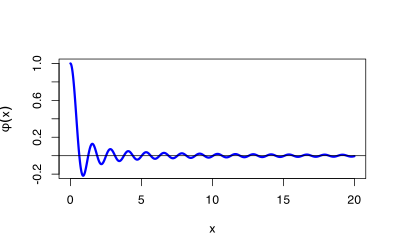
\includegraphics[keepaspectratio]{index_files/mediabag/lectures/L08-is-1_files/figure-pdf/importance-1.pdf}}

We can see that what happens for small \(x\) -- say, for \(x\) between 0
and 2, or so -- will have an important effect on the value of
\(\Exg \phi(X)\), because that where \(\phi\) has the biggest (absolute)
values. But what happens for large \(x\) -- say for \(x \geq 10\) or so
-- will be much less important for estimating \(\Exg\phi(X)\). So it
seems wasteful to have all values in \([0, 20]\) to be sampled equally,
and it would seem to make sense to take more samples from small values
of \(x\).

This is all very well in practice, but how exactly should we down-weight
those over-sampled areas?

Think about estimating \(\Exg \phi(X)\). Let's assume that \(X\) is
continuous with probability density function \(f\). (Throughout this
lecture and the next, we will assume all our random variables are
continuous. The arguments for discrete random variables are very similar
-- just swap probability density functions with probability mass
functions and integrals with sums. You can fill in the details yourself,
if you like.) Then we are trying to estimate
\[ \Exg \phi(X) = \int_{-\infty}^{+\infty} \phi(x)\,f(x)\,\mathrm{d}x = \int_{-\infty}^{+\infty} \phi(y)\,f(y)\,\mathrm{d}y . \]
(In the second equality, we merely changed the ``dummy variable'' from
\(x\) to \(y\), as we are at liberty to do.)

Now suppose we sample from some other continuous distribution \(Y\),
with PDF \(g\). If we estimate \(\Exg \psi(Y)\), say, for some function
\(\psi\), then we are estimating
\[\Exg \psi(Y) = \int_{-\infty}^{+\infty} \psi(y)\,g(y) \, \mathrm{d}y = \int_{-\infty}^{+\infty} \psi(x)\,g(x) \, \mathrm{d}x . \]

But we want to be estimating \(\Exg\phi(X)\), not \(\Exg\psi(Y)\). So we
will need to pick \(\psi\) such that
\[ \Exg \phi(X) = \int_{-\infty}^{+\infty} \phi(y)\,f(y)\,\mathrm{d}y = \int_{-\infty}^{+\infty} \psi(y)\,g(y) \, \mathrm{d}y = \Exg \psi(Y) . \]
So we need to pick \(\psi\) such that \(\phi(y)\,f(y) = \psi(y)\,g(y)\).
That means that we should take
\[\psi(y) = \frac{\phi(y) f(y)}{g(y)} = \frac{f(y)}{g(y)}\,\phi(y). \]

So we could build a Monte Carlo estimate for \(\Exg \phi(X)\) instead as
a Monte Carlo estimate for
\[ \Exg \psi(Y) = \Exg \left(\frac{f(Y)}{g(Y)}\,\phi(Y) \right) . \]

There is one other thing: we need to be careful of division by \(0\)
errors. So we should make sure that \(g\) is only 0 when \(f\) is 0. In
other words, if it's possible for \(X\) to take some value, then it must
be possible for \(Y\) to take that value too.

We are finally ready to define our estimator.

\begin{definition}[]\protect\hypertarget{def-IS}{}\label{def-IS}

Let \(X\) be a continuous random variable with probability density
function \(f\), let \(\phi\) be a function, and write
\(\theta = \Exg\phi(X)\). Let \(Y\) be a continuous random variable with
probability desnity function \(g\), where \(g(y) > 0\) for all \(y\)
where \(f(y) > 0\). Then the \textbf{importance sampling Monte Carlo
estimator} \(\widehat\theta_n^{\mathrm{IS}}\) of \(\theta\) is
\[ \widehat{\theta}_n^{\mathrm{IS}} = \frac{1}{n} \sum_{i=1}^{n} \frac{f(Y_i)}{g(Y_i)}\, \phi(Y_i)   ,\]
where \(Y_1, Y_2, \dots, Y_n\) are independent random samples from
\(Y\).

\end{definition}

We can think of this as taking a weighted mean of the \(\phi(Y_i)\)s,
where the weights are \(f(Y_i)/g(Y_i)\). So if a value \(y\) is more
likely under \(Y\) than under \(X\), then \(g(y)\) is big compared to
\(f(y)\), so \(f(y)/g(y)\) is small, and \(y\) gets a low weight. If a
value \(y\) is less likely under \(Y\) than under \(X\), then \(g(y)\)
is small compared to \(f(y)\), so \(f(y) / g(y)\) is big, and it gets a
high weight. Thus we see that the weighting compensates for values that
are likely to be over- or under-sampled.

\section{Example}\label{example}

\begin{example}[]\protect\hypertarget{exm-IS1}{}\label{exm-IS1}

Let \(X \sim \operatorname{N}(0,1)\) be a standard normal. Suppose we
want to estimate \(\mathbb P(X > 4)\). We could do this the standard
Monte Carlo way by sampling from \(X\) itself.
\[ \widehat{\theta}_n^{\mathrm{MS}} = \frac{1}{n} \sum_{i=1}^n \mathbb I_{[4,\infty)}(X_i) . \]

However, this will not be a good estimator. To see the problem, lets run
this with \(n = 100\,000 = 10^5\) samples, but do it 10 times, and see
what all the estimates are.

\begin{Shaded}
\begin{Highlighting}[]
\NormalTok{n }\OtherTok{\textless{}{-}} \FloatTok{1e5}
\NormalTok{MCest }\OtherTok{\textless{}{-}} \FunctionTok{rep}\NormalTok{(}\DecValTok{0}\NormalTok{, }\DecValTok{10}\NormalTok{)}
\ControlFlowTok{for}\NormalTok{ (i }\ControlFlowTok{in} \DecValTok{1}\SpecialCharTok{:}\DecValTok{10}\NormalTok{) MCest[i] }\OtherTok{\textless{}{-}} \FunctionTok{mean}\NormalTok{(}\FunctionTok{rnorm}\NormalTok{(n) }\SpecialCharTok{\textgreater{}} \DecValTok{4}\NormalTok{)}
\NormalTok{MCest}
\end{Highlighting}
\end{Shaded}

\begin{verbatim}
 [1] 4e-05 3e-05 3e-05 7e-05 1e-05 5e-05 6e-05 1e-05 5e-05 1e-05
\end{verbatim}

We see a big range of values. I get different results each time I run
it, but anything between \(1 \times 10^{-5}\) and \(8 \times 10^{-5}\),
and even \(0\), comes out fairly regularly as the estimate. The problem
is that \(X > 4\) is a very rare event -- it only comes out a handful of
times (perhaps 0 to 8) out of the 100,000 samples. This means our
estimate is (on average) quite inaccurate.

It would be better not to sample from \(X\), but rather to sample from a
distribution that is greater than 4 a better proportion of the time. We
could try anything for this distribution \(Y\), but to keep things
simple, I'm going to stick with a normal distribution with standard
deviation 1. I'll want to increase the mean, though, so that we sample
values bigger than 4 more often. Let's try importance sampling with
\(Y \sim \operatorname{N}(4,1)\).

The PDFs of \(X \sim \operatorname{N}(0,1)\) and
\(Y \sim \operatorname{N}(4,1)\) are
\[f(x) = \frac{1}{\sqrt{2\pi}} \exp\big(-\tfrac12 x^2\big) \qquad g(y) = \frac{1}{\sqrt{2\pi}} \exp\big(-\tfrac12 (y-4)^2\big) , \]
so the relevant weighting of a sample \(y\) is
\[ \frac{f(y)}{g(y)} = \frac{\exp\big(-\tfrac12 y^2\big)}{\exp\big(-\tfrac12 (y-4)^2\big)} = \exp \big(\tfrac12\big(-y^2 + (y-4)^2\big)\big) = \exp(-4y+8) .  \]
So our importance sampling estimate will be
\[ \widehat{\theta}_n^{\mathrm{IS}} = \frac{1}{n} \sum_{i=1}^n \mathrm{e}^{-4Y_i +8} \, \mathbb I_{[4,\infty)}(Y_i) . \]

Let's try this in R. Although we could use the function
\(\mathrm{e}^{-4y+8}\) for the weights, I'll do this by using the ratios
of the PDFs directly in R (just in case I made a mistake\ldots).

\begin{Shaded}
\begin{Highlighting}[]
\NormalTok{n }\OtherTok{\textless{}{-}} \FloatTok{1e5}
\NormalTok{pdf\_x }\OtherTok{\textless{}{-}} \ControlFlowTok{function}\NormalTok{(y) }\FunctionTok{dnorm}\NormalTok{(y, }\DecValTok{0}\NormalTok{, }\DecValTok{1}\NormalTok{)}
\NormalTok{pdf\_y }\OtherTok{\textless{}{-}} \ControlFlowTok{function}\NormalTok{(y) }\FunctionTok{dnorm}\NormalTok{(y, }\DecValTok{4}\NormalTok{, }\DecValTok{1}\NormalTok{)}
\NormalTok{samples\_y }\OtherTok{\textless{}{-}} \FunctionTok{rnorm}\NormalTok{(n, }\DecValTok{4}\NormalTok{, }\DecValTok{1}\NormalTok{)}
\NormalTok{ISest }\OtherTok{\textless{}{-}} \FunctionTok{mean}\NormalTok{((}\FunctionTok{pdf\_x}\NormalTok{(samples\_y) }\SpecialCharTok{/} \FunctionTok{pdf\_y}\NormalTok{(samples\_y)) }\SpecialCharTok{*}\NormalTok{ (samples\_y }\SpecialCharTok{\textgreater{}} \DecValTok{4}\NormalTok{))}
\NormalTok{ISest}
\end{Highlighting}
\end{Shaded}

\begin{verbatim}
[1] 3.163129e-05
\end{verbatim}

\end{example}

\section{Errors in importance
sampling}\label{errors-in-importance-sampling}

The following theorem should not by now be a surprise.

\begin{theorem}[]\protect\hypertarget{thm-Iserr}{}\label{thm-Iserr}

Let \(X\) be a continuous random variable with probability density
function \(f\), let \(\phi\) be a function, and write
\(\theta = \Exg\phi(X)\). Let \(Y\) another continuous random variable
with probability density function with probability density function
\(g\), such that \(g(y) = 0\) only when \(f(y) = 0\). Let
\[ \widehat{\theta}_n^{\mathrm{IS}} = \frac{1}{n} \sum_{i=1}^n \frac{f(Y_i)}{g(Y_i)}\,\phi(Y_i)  \]
be the importance sampling Monte Carlo estimator of \(\theta\). Then:

\begin{enumerate}
\def\labelenumi{\arabic{enumi}.}
\item
  \(\widehat{\theta}_n^{\mathrm{IS}}\) is unbiased, in that
  \(\operatorname{bias}\big(\widehat{\theta}_n^{\mathrm{IS}}\big) = 0\).
\item
  The variance of of \(\widehat{\theta}_n^{\mathrm{IS}}\) is
  \[ \operatorname{Var}\big(\widehat{\theta}_n^{\mathrm{IS}}\big) = \frac{1}{n} \operatorname{Var}\left( \frac{f(Y)}{g(Y)}\,\phi(Y) \right). \]
\item
  The mean-square error of \(\widehat{\theta}_n^{\mathrm{IS}}\) is
  \[ \operatorname{MSE}\big(\widehat{\theta}_n^{\mathrm{IS}}\big) = \frac{1}{n} \operatorname{Var}\left( \frac{f(Y)}{g(Y)}\,\phi(Y) \right) . \]
\item
  The root-mean-square error of \(\widehat{\theta}_n^{\mathrm{IS}}\) is
  \[ \operatorname{RMSE}\big(\widehat{\theta}_n^{\mathrm{IS}}\big) = \frac{1}{\sqrt{n}} \,\sqrt{\operatorname{Var}\left( \frac{f(Y)}{g(Y)}\,\phi(Y) \right)}. \]
\end{enumerate}

\end{theorem}

\begin{proof}
Part 1 follows essentially the same argument as our discussion at the
beginning of this lecture. We have
\[ \Ex \left( \frac{1}{n} \sum_{i=1}^n \frac{f(Y_i)}{g(Y_i)}\,\phi(Y_i) \right) = \frac{1}{n}\, n\, \Ex \left(\frac{f(Y)}{g(Y)}\,\phi(Y)\right) = \Ex \left(\frac{f(Y)}{g(Y)}\,\phi(Y)\right) . \]
But
\[ \Ex \left(\frac{f(Y)}{g(Y)}\,\phi(Y)\right) = \int_{-\infty}^{+\infty} \frac{f(y)}{g(y)}\,\phi(y)\,g(y)\,\mathrm{d}y = \int_{-\infty}^{+\infty} \phi(y) \, f(y) \, \mathrm{d}y = \Exg \phi(X) . \]
This last step is because \(f\) is the PDF of \(X\); it doesn't matter
whether the dummy variable in the integration is \(x\) or \(y\). Hence
the estimator is unbiased.

Parts 2 to 4 follow in the usual way.
\end{proof}

As we are now used to, we can estimate the variance using the sample
variance.

\begin{example}[]\protect\hypertarget{exm-IS2}{}\label{exm-IS2}

We continue Example~\ref{exm-IS1}, where we are estimating
\(\mathbb P(X > 4)\) for \(X \sim \operatorname{N}(0,1)\).

For the standard Monte Carlo method, we estimate the root-mean-square
error as

\begin{Shaded}
\begin{Highlighting}[]
\NormalTok{n }\OtherTok{\textless{}{-}} \FloatTok{1e5}
\NormalTok{MC\_MSE }\OtherTok{\textless{}{-}} \FunctionTok{var}\NormalTok{(}\FunctionTok{rnorm}\NormalTok{(n) }\SpecialCharTok{\textgreater{}} \DecValTok{4}\NormalTok{) }\SpecialCharTok{/}\NormalTok{ n}
\FunctionTok{sqrt}\NormalTok{(MC\_MSE)}
\end{Highlighting}
\end{Shaded}

\begin{verbatim}
[1] 1.732033e-05
\end{verbatim}

As before, this still varies a lot, but it seems to usually be about
\(2 \times 10^{-5}\).

For the importance sampling method, we estimate the mean-square error as

\begin{Shaded}
\begin{Highlighting}[]
\NormalTok{n }\OtherTok{\textless{}{-}} \FloatTok{1e5}
\NormalTok{pdf\_x }\OtherTok{\textless{}{-}} \ControlFlowTok{function}\NormalTok{(x) }\FunctionTok{dnorm}\NormalTok{(x, }\DecValTok{0}\NormalTok{, }\DecValTok{1}\NormalTok{)}
\NormalTok{pdf\_y }\OtherTok{\textless{}{-}} \ControlFlowTok{function}\NormalTok{(y) }\FunctionTok{dnorm}\NormalTok{(y, }\DecValTok{4}\NormalTok{, }\DecValTok{1}\NormalTok{)}
\NormalTok{samples\_y }\OtherTok{\textless{}{-}} \FunctionTok{rnorm}\NormalTok{(n, }\DecValTok{4}\NormalTok{, }\DecValTok{1}\NormalTok{)}
\NormalTok{IS\_MSE }\OtherTok{\textless{}{-}} \FunctionTok{var}\NormalTok{((}\FunctionTok{pdf\_x}\NormalTok{(samples\_y) }\SpecialCharTok{/} \FunctionTok{pdf\_y}\NormalTok{(samples\_y)) }\SpecialCharTok{*}\NormalTok{ (samples\_y }\SpecialCharTok{\textgreater{}} \DecValTok{4}\NormalTok{)) }\SpecialCharTok{/}\NormalTok{ n}
\FunctionTok{sqrt}\NormalTok{(IS\_MSE)}
\end{Highlighting}
\end{Shaded}

\begin{verbatim}
[1] 2.129446e-07
\end{verbatim}

This is about \(2 \times 10^{-7}\). This is about 100 times smaller than
for the standard method: equivalent to taking about 10,000 times as many
samples! That's a huge improvement, which demonstrates the power of
importance sampling.

\end{example}

\textbf{Next time:} \emph{We continue our study of importance sampling
-- and complete our study of Monte Carlo estimation, for now -- by
considering how to pick a good distribution \(Y\).}

\textbf{Summary:}

\begin{itemize}
\item
  Importance sampling estimates \(\Exg \phi(X)\) by sampling from a
  different distribution \(Y\).
\item
  The importance sampling estimator is
  \({\displaystyle \widehat{\theta}_n^{\mathrm{IS}} = \frac{1}{n} \sum_{i=1}^n \frac{f(Y_i)}{g(Y_i)}\,\phi(Y_i)}\).
\item
  The importance sampling estimator is unbiased with mean-square error
  \[ \operatorname{MSE}\big(\widehat{\theta}_n^{\mathrm{IS}}\big) = \frac{1}{n} \operatorname{Var}\left( \frac{f(Y)}{g(Y)}\,\phi(Y) \right) . \]
\end{itemize}

\textbf{\hyperref[solutions]{Solutions}} are now available for Problem
Sheet 1.

\textbf{Read more:}
\href{https://leeds.primo.exlibrisgroup.com/permalink/44LEE_INST/1fj430b/cdi_askewsholts_vlebooks_9781118728031}{Voss,
\emph{An Introduction to Statistical Computing}}, Subsection 3.3.1.

\chapter{Importance sampling II}\label{importance-sampling-ii}

\[ \]

\section{Picking a good distribution}\label{picking-a-good-distribution}

Let's remind ourselves where we've got to on importance sampling.

\begin{itemize}
\item
  We want to estimate \(\Exg \phi(X)\).
\item
  Rather than sampling from \(X\), with PDF \(f\), we instead sample
  from a different distribution \(Y\), with PDF \(g\).
\item
  The estimator is
  \({\displaystyle \widehat\theta_n^{\text{IS}} = \frac{1}{n} \sum_{i=1}^n \frac{f(Y_i)}{g(Y_i)} \, \phi(Y_i) .}\)
\end{itemize}

We've seen that importance sampling can be a very powerful tool, when
used well. But how should pick a good distribution \(Y\) to sample from?

Let's examine the mean-square error more carefully:
\[ \operatorname{MSE}\big(\widehat{\theta}_n^{\mathrm{IS}}\big) = \frac{1}{n} \operatorname{Var}\left( \frac{f(Y)}{g(Y)}\,\phi(Y) \right) . \]
So our goal is to try and pick \(Y\) such that
\(\frac{f(Y)}{g(Y)}\phi(Y)\) has low variance. We also, of course, want
to be able to sample from \(Y\).

The best possible choice, then, would be to pick \(Y\) such that
\(\frac{f(Y)}{g(Y)}\phi(Y)\) is constant -- and therefore has zero
variance! If \(\phi\) is non-negative, then it seems like we should pick
\(Y\) such that its probability density function is
\(g(y) \propto f(y)\phi(y)\). (Here, \(\propto\) is the ``proportional
to'' symbol.) That is, to have \[ g(y) = \frac{1}{Z} f(y)\phi(y) , \]
for some constant \(Z\). Then \(\frac{f(Y)}{g(Y)}\phi(Y) = Z\) is a
constant, has zero variance, and we have a perfect estimator!

What is this constant \(Z\)? Well, \(g\) is a PDF, so it has to
integrate to 1. So we will need to have
\[ 1 = \int_{-\infty}^{+\infty} g(y)\, \mathrm{d}y = \int_{-\infty}^{+\infty} \frac{1}{Z} f(y)\phi(y) \, \mathrm{d}y = \frac{1}{Z} \int_{-\infty}^{+\infty} f(x)\phi(x) \, \mathrm{d}x = \frac{1}{Z} \Exg\phi(X) . \]
(We did the ``switching the dummy variable from \(y\) to \(x\)'' thing
again.) So \(Z = \Exg \phi(X)\). But that's no good:
\(\theta = \Exg \phi(X)\) was the thing we were trying to estimate in
the first place. If we knew that, we wouldn't have to do Monte Carlo
estimation to start with!

So, as much as we would like to, we can't use this ``perfect'' ideal
distribution \(Y\). More generally, if \(\phi\) is not always
non-negative, it can be shown that
\(g(y) \propto f(y)\,|\phi(y)| = |f(x)\,\phi(x)|\) would be the best
possible distribution, but this has the same problems.

However, we can still be guided by this idea -- we would like \(g(y)\)
to be as close to proportional to \(f(y) \phi(y)\) (or
\(|f(y) \phi(y)|\)) as we can manage, so that
\(\frac{f(y)}{g(y)}\phi(y)\) is close to being constant, so hopefully
has low variance. This tells us that \(Y\) should be likely -- that is,
\(g(y)\) should be big -- where both \(f\) and \(|\phi|\) are both big
-- that is, where \(X\) is likely and also \(\phi\) is big in absolute
value. While \(Y\) should be unlikely where both \(X\) is unlikely and
\(\phi\) is small in absolute value.

\begin{example}[]\protect\hypertarget{exm-IS3}{}\label{exm-IS3}

Let's look again at Example~\ref{exm-IS1} (continued in
Example~\ref{exm-IS2}), where we wanted to estimate
\(\mathbb P(X > 4) = \Exg\Ind_{(4,\infty)}(X)\) for
\(X \sim \operatorname{N}(0,1)\). We found are estimator was enormously
improved when we used instead \(Y \sim \operatorname{N}(4,1)\).

In the figure below, the blue line is
\[f(y)\,\phi(y) = f(y)\,\Ind_{(4,\infty)}(y) = \begin{cases} \displaystyle\frac{1}{\sqrt{2\pi}} \,\mathrm{e}^{-y^2/2} & y > 4 \\ 0 & y \leq 4 \end{cases} \]
(scaled up, otherwise it would be so close to the axis line you wouldn't
see it).

The black line is the PDF \(f(y)\) of the original distribution
\(X \sim \operatorname{N}(0,1)\), while the red line is the PDF \(g(y)\)
of our importance distribution \(Y \sim \operatorname{N}(4,1)\).

\begin{Shaded}
\begin{Highlighting}[]
\FunctionTok{curve}\NormalTok{(}
  \FunctionTok{dnorm}\NormalTok{(x, }\DecValTok{0}\NormalTok{, }\DecValTok{1}\NormalTok{), }\AttributeTok{n =} \DecValTok{1001}\NormalTok{, }\AttributeTok{from =} \SpecialCharTok{{-}}\FloatTok{2.5}\NormalTok{, }\AttributeTok{to =} \FloatTok{7.5}\NormalTok{,}
  \AttributeTok{col =} \StringTok{"black"}\NormalTok{, }\AttributeTok{lwd =} \DecValTok{2}\NormalTok{,}
  \AttributeTok{xlim =} \FunctionTok{c}\NormalTok{(}\SpecialCharTok{{-}}\DecValTok{2}\NormalTok{, }\DecValTok{7}\NormalTok{), }\AttributeTok{xlab =} \StringTok{"y"}\NormalTok{, }\AttributeTok{ylim =} \FunctionTok{c}\NormalTok{(}\DecValTok{0}\NormalTok{, }\FloatTok{0.7}\NormalTok{), }\AttributeTok{ylab =} \StringTok{""}
\NormalTok{)}
\FunctionTok{curve}\NormalTok{(}
  \FunctionTok{dnorm}\NormalTok{(x, }\DecValTok{4}\NormalTok{, }\DecValTok{1}\NormalTok{), }\AttributeTok{n =} \DecValTok{1001}\NormalTok{, }\AttributeTok{from =} \SpecialCharTok{{-}}\FloatTok{2.5}\NormalTok{, }\AttributeTok{to =} \FloatTok{7.5}\NormalTok{,}
  \AttributeTok{add =} \ConstantTok{TRUE}\NormalTok{, }\AttributeTok{col =} \StringTok{"red"}\NormalTok{, }\AttributeTok{lwd =} \DecValTok{3}\NormalTok{,}
\NormalTok{)}
\FunctionTok{curve}\NormalTok{(}
  \FunctionTok{dnorm}\NormalTok{(x, }\DecValTok{0}\NormalTok{, }\DecValTok{1}\NormalTok{) }\SpecialCharTok{*}\NormalTok{ (x }\SpecialCharTok{\textgreater{}} \DecValTok{4}\NormalTok{) }\SpecialCharTok{*} \DecValTok{5000}\NormalTok{, }\AttributeTok{n =} \DecValTok{1001}\NormalTok{, }\AttributeTok{from =} \SpecialCharTok{{-}}\FloatTok{2.5}\NormalTok{, }\AttributeTok{to =} \FloatTok{7.5}\NormalTok{,}
  \AttributeTok{add =} \ConstantTok{TRUE}\NormalTok{, }\AttributeTok{col =} \StringTok{"blue"}\NormalTok{, }\AttributeTok{lwd =} \DecValTok{3}
\NormalTok{)}
\FunctionTok{legend}\NormalTok{(}
  \StringTok{"topright"}\NormalTok{,}
  \FunctionTok{c}\NormalTok{(}\FunctionTok{expression}\NormalTok{(}\FunctionTok{paste}\NormalTok{(}\StringTok{"f(y)"}\NormalTok{, varphi, }\StringTok{"(y) [scaled]"}\NormalTok{)), }\StringTok{"N(0, 1)"}\NormalTok{, }\StringTok{"N(4, 1)"}\NormalTok{),}
  \AttributeTok{lwd =} \FunctionTok{c}\NormalTok{(}\DecValTok{3}\NormalTok{, }\DecValTok{2}\NormalTok{, }\DecValTok{3}\NormalTok{), }\AttributeTok{col =} \FunctionTok{c}\NormalTok{(}\StringTok{"blue"}\NormalTok{, }\StringTok{"black"}\NormalTok{, }\StringTok{"red"}\NormalTok{)}
\NormalTok{)}
\end{Highlighting}
\end{Shaded}

\pandocbounded{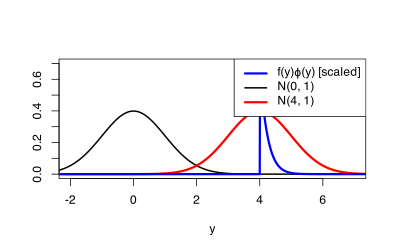
\includegraphics[keepaspectratio]{index_files/mediabag/lectures/L09-is-2_files/figure-pdf/propto-1.pdf}}

We have noted that a good distribution will have a PDF that is big when
\(f(x)\phi(x)\) (the blue line) is big. Clearly the red line is much
better at this then the black line, which is why the importance sampling
method was so much better here.

There's scope to do better here, though. Perhaps an asymmetric
distribution with a much more quickly-decaying left-tail might be good
-- for example, a shifted exponential
\(4 + \operatorname{Exp}(\lambda)\) might be worth investigating. Or a
thinner, spikier distribution, such as a normal with smaller standard
deviation. In both cases, though, we have to be careful -- because it's
the ratio \(f(y)/g(y)\), we still have to be a bit careful about what
happens when both \(f(y)\) and \(g(y)\) are small \emph{absolutely}, in
case one is \emph{proportionally} much bigger than the other.

\end{example}

Aside from the exact theory, in the absence of any better idea, choosing
\(Y\) to be ``in the same distribution family as \(X\) but with
different parameters'' is often a reasonable thing to try. For example:

\begin{itemize}
\item
  If \(X \sim \operatorname{N}(\mu, \sigma^2)\), then try
  \(Y \sim \operatorname{N}(\nu, \sigma^2)\) for some other value
  \(\nu\).
\item
  If \(X \sim \operatorname{Exp}(\lambda)\), then try
  \(Y \sim \operatorname{Exp}(\mu)\) for some other value \(\mu\).
\end{itemize}

\section{Bonus example}\label{bonus-example}

\begin{example}[]\protect\hypertarget{exm-ISnew}{}\label{exm-ISnew}

\emph{Let} \(X \sim \operatorname{U}[0, 10]\) be an uniform
distribution, so \(f(x) = \frac{1}{10}\) for \(0 \leq x \leq 10\), and
let \(\phi(x) = \mathrm{e}^{-|x-8|}\). Estimate \(\Exg\phi(X)\).

The standard Monte Carlo estimator and its RMSE are as follows

\begin{Shaded}
\begin{Highlighting}[]
\NormalTok{phi }\OtherTok{\textless{}{-}} \ControlFlowTok{function}\NormalTok{(x) }\FunctionTok{exp}\NormalTok{(}\SpecialCharTok{{-}}\FunctionTok{abs}\NormalTok{(x }\SpecialCharTok{{-}} \DecValTok{8}\NormalTok{))}
\NormalTok{n }\OtherTok{\textless{}{-}} \FloatTok{1e6}
\NormalTok{samples }\OtherTok{\textless{}{-}} \FunctionTok{runif}\NormalTok{(n, }\DecValTok{0}\NormalTok{, }\DecValTok{10}\NormalTok{)}
\NormalTok{MCest }\OtherTok{\textless{}{-}} \FunctionTok{mean}\NormalTok{(}\FunctionTok{phi}\NormalTok{(samples))}
\NormalTok{MC\_MSE }\OtherTok{\textless{}{-}} \FunctionTok{var}\NormalTok{(}\FunctionTok{phi}\NormalTok{(samples)) }\SpecialCharTok{/}\NormalTok{ n}
\FunctionTok{c}\NormalTok{(MCest, }\FunctionTok{sqrt}\NormalTok{(MC\_MSE))}
\end{Highlighting}
\end{Shaded}

\begin{verbatim}
[1] 0.1865579341 0.0002537701
\end{verbatim}

Maybe we can improve on this using importance sampling. Let's have a
look at a graph of \(f(y)\,\phi(y)\) (blue line).

\begin{Shaded}
\begin{Highlighting}[]
\FunctionTok{curve}\NormalTok{(}
  \FunctionTok{dunif}\NormalTok{(x, }\DecValTok{0}\NormalTok{, }\DecValTok{10}\NormalTok{) }\SpecialCharTok{*} \FunctionTok{exp}\NormalTok{(}\SpecialCharTok{{-}}\FunctionTok{abs}\NormalTok{(x }\SpecialCharTok{{-}} \DecValTok{8}\NormalTok{)), }\AttributeTok{n =} \DecValTok{1001}\NormalTok{, }\AttributeTok{from =} \SpecialCharTok{{-}}\DecValTok{1}\NormalTok{, }\AttributeTok{to =} \DecValTok{11}\NormalTok{,}
  \AttributeTok{col =} \StringTok{"blue"}\NormalTok{, }\AttributeTok{lwd =} \DecValTok{3}\NormalTok{,}
  \AttributeTok{xlim =} \FunctionTok{c}\NormalTok{(}\DecValTok{0}\NormalTok{, }\DecValTok{10}\NormalTok{), }\AttributeTok{xlab =} \StringTok{"y"}\NormalTok{, }\AttributeTok{ylab =} \StringTok{""}
\NormalTok{)}
\FunctionTok{curve}\NormalTok{(}
  \FunctionTok{dnorm}\NormalTok{(x, }\DecValTok{8}\NormalTok{, }\DecValTok{2}\NormalTok{)}\SpecialCharTok{*}\FloatTok{0.36}\NormalTok{, }\AttributeTok{n =} \DecValTok{1001}\NormalTok{, }\AttributeTok{from =} \SpecialCharTok{{-}}\DecValTok{1}\NormalTok{, }\AttributeTok{to =} \DecValTok{11}\NormalTok{,}
  \AttributeTok{add =} \ConstantTok{TRUE}\NormalTok{, }\AttributeTok{col =} \StringTok{"red"}\NormalTok{, }\AttributeTok{lwd =} \DecValTok{2}\NormalTok{,}
\NormalTok{)}
\FunctionTok{legend}\NormalTok{(}
  \StringTok{"topleft"}\NormalTok{,}
  \FunctionTok{c}\NormalTok{(}\FunctionTok{expression}\NormalTok{(}\FunctionTok{paste}\NormalTok{(}\StringTok{"f(y)"}\NormalTok{, varphi, }\StringTok{"(y)"}\NormalTok{)), }\StringTok{"N(8, 4) [scaled]"}\NormalTok{),}
  \AttributeTok{lwd =} \FunctionTok{c}\NormalTok{(}\DecValTok{3}\NormalTok{, }\DecValTok{2}\NormalTok{), }\AttributeTok{col =} \FunctionTok{c}\NormalTok{(}\StringTok{"blue"}\NormalTok{, }\StringTok{"red"}\NormalTok{)}
\NormalTok{)}
\end{Highlighting}
\end{Shaded}

\pandocbounded{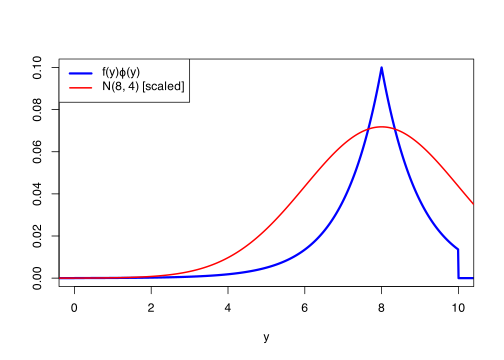
\includegraphics[keepaspectratio]{index_files/mediabag/lectures/L09-is-2_files/figure-pdf/propto2-1.pdf}}

After some experimentation, I decided that
\(Y \sim \operatorname{N}(8, 2^2)\) (red line; not to same scale) seemed
to work quite well, in \(g(y)\) being roughly proportional to
\(f(y)\,\phi(y)\). (Maybe reducing the standard deviation a bit more, to
around 1.6, to get the red curve a bit tighter, might have done a little
bit better still.)

The following graph shows \(\frac{f(y)}{g(y)} \phi(y)\), and shows that
the graph is not \emph{too} pointy, so should have reasonably small
variance.

\begin{Shaded}
\begin{Highlighting}[]
\FunctionTok{curve}\NormalTok{(}
  \FunctionTok{dunif}\NormalTok{(x, }\DecValTok{0}\NormalTok{, }\DecValTok{10}\NormalTok{) }\SpecialCharTok{*} \FunctionTok{exp}\NormalTok{(}\SpecialCharTok{{-}}\FunctionTok{abs}\NormalTok{(x }\SpecialCharTok{{-}} \DecValTok{8}\NormalTok{)) }\SpecialCharTok{/} \FunctionTok{dnorm}\NormalTok{(x, }\DecValTok{8}\NormalTok{, }\DecValTok{2}\NormalTok{), }\AttributeTok{n =} \DecValTok{1001}\NormalTok{, }\AttributeTok{from =} \SpecialCharTok{{-}}\DecValTok{2}\NormalTok{, }\AttributeTok{to =} \DecValTok{12}\NormalTok{,}
  \AttributeTok{col =} \StringTok{"red"}\NormalTok{, }\AttributeTok{lwd =} \DecValTok{3}\NormalTok{,}
  \AttributeTok{xlim =} \FunctionTok{c}\NormalTok{(}\SpecialCharTok{{-}}\DecValTok{1}\NormalTok{, }\DecValTok{11}\NormalTok{), }\AttributeTok{xlab =} \StringTok{"y"}\NormalTok{, }\AttributeTok{ylab =} \StringTok{""}
\NormalTok{)}
\end{Highlighting}
\end{Shaded}

\pandocbounded{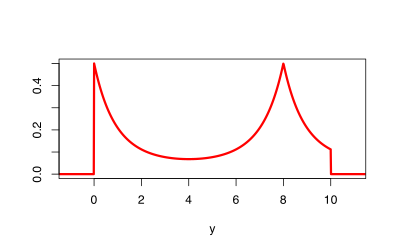
\includegraphics[keepaspectratio]{index_files/mediabag/lectures/L09-is-2_files/figure-pdf/propto3-1.pdf}}

So our importance sampling estimate is as follows.

\begin{Shaded}
\begin{Highlighting}[]
\NormalTok{phi }\OtherTok{\textless{}{-}} \ControlFlowTok{function}\NormalTok{(x) }\FunctionTok{exp}\NormalTok{(}\SpecialCharTok{{-}}\FunctionTok{abs}\NormalTok{(x }\SpecialCharTok{{-}} \DecValTok{8}\NormalTok{))}
\NormalTok{pdf\_x }\OtherTok{\textless{}{-}} \ControlFlowTok{function}\NormalTok{(x) }\FunctionTok{dunif}\NormalTok{(x, }\DecValTok{0}\NormalTok{, }\DecValTok{10}\NormalTok{)}
\NormalTok{pdf\_y }\OtherTok{\textless{}{-}} \ControlFlowTok{function}\NormalTok{(y) }\FunctionTok{dnorm}\NormalTok{(y, }\DecValTok{8}\NormalTok{, }\DecValTok{2}\NormalTok{)}

\NormalTok{n }\OtherTok{\textless{}{-}} \FloatTok{1e6}
\NormalTok{samples }\OtherTok{\textless{}{-}} \FunctionTok{rnorm}\NormalTok{(n, }\DecValTok{8}\NormalTok{, }\DecValTok{2}\NormalTok{)}
\NormalTok{ISest }\OtherTok{\textless{}{-}} \FunctionTok{mean}\NormalTok{((}\FunctionTok{pdf\_x}\NormalTok{(samples) }\SpecialCharTok{/} \FunctionTok{pdf\_y}\NormalTok{(samples)) }\SpecialCharTok{*} \FunctionTok{phi}\NormalTok{(samples))}
\NormalTok{IS\_MSE }\OtherTok{\textless{}{-}} \FunctionTok{var}\NormalTok{((}\FunctionTok{pdf\_x}\NormalTok{(samples) }\SpecialCharTok{/} \FunctionTok{pdf\_y}\NormalTok{(samples)) }\SpecialCharTok{*} \FunctionTok{phi}\NormalTok{(samples)) }\SpecialCharTok{/}\NormalTok{ n}
\FunctionTok{c}\NormalTok{(ISest, }\FunctionTok{sqrt}\NormalTok{(IS\_MSE))}
\end{Highlighting}
\end{Shaded}

\begin{verbatim}
[1] 0.1863512119 0.0001351446
\end{verbatim}

We see that the RMSE has roughly halved, which is the equivalent of
taking four times as many samples.

\end{example}

\section{Summary of Part I}\label{summary-of-part-i}

This is our last lecture on Monte Carlo estimation -- at least for now,
and at least in its standard form. So let's end this section of the
module by summarising the estimators we have learned about. We have been
learning how to estimate \(\theta = \Exg \phi(X)\)

\begin{itemize}
\item
  The \textbf{standard Monte Carlo estimator} simple takes a sample mean
  of \(\phi(X_i)\), where \(X_i\) are independent random samples from
  \(X\).
\item
  The \textbf{control variate} Monte Carlo estimator ``anchors'' the
  estimator to some known value \(\eta = \Exg \psi(X)\), for a function
  \(\psi\) that is ``similar to \(\phi\), but easier to calculate the
  expectation exactly''.
\item
  The \textbf{antithetic variables} Monte Carlo estimator uses pairs of
  samples \((X_i, X'_i)\) that both have the same distribution as \(X\),
  but where \(\phi(X)\) and \(\phi(X')\) have negative correlation
  \(\rho < 0\).
\item
  The \textbf{importance sampling} Monte Carlo estimator samples not
  from \(X\), with PDF \(f\), but from a different distribution \(Y\),
  with PDF \(Y\). The distribution \(Y\) is chosen to oversample from
  the most important values, but then gives lower weight to those
  samples.
\end{itemize}

\begin{longtable}[]{@{}
  >{\centering\arraybackslash}p{(\linewidth - 4\tabcolsep) * \real{0.3333}}
  >{\centering\arraybackslash}p{(\linewidth - 4\tabcolsep) * \real{0.3333}}
  >{\centering\arraybackslash}p{(\linewidth - 4\tabcolsep) * \real{0.3333}}@{}}
\toprule\noalign{}
\begin{minipage}[b]{\linewidth}\centering
\end{minipage} & \begin{minipage}[b]{\linewidth}\centering
\textbf{Estimator}
\end{minipage} & \begin{minipage}[b]{\linewidth}\centering
\textbf{MSE}
\end{minipage} \\
\midrule\noalign{}
\endhead
\bottomrule\noalign{}
\endlastfoot
\textbf{Standard Monte Carlo} &
\({\displaystyle\frac{1}{n} \sum_{i=1}^n \phi(X_i)}\) &
\({\displaystyle\frac{1}{n} \operatorname{Var}\big(\phi(X)\big)}\) \\
\textbf{Control variate} &
\({\displaystyle\frac{1}{n} \sum_{i=1}^n \big(\phi(X_i) - \psi(X_i)\big)} + \eta\)
&
\({\displaystyle\frac{1}{n} \operatorname{Var}\big(\phi(X_i) - \psi(X_i)\big)}\) \\
\textbf{Antithetic variables} &
\({\displaystyle\frac{1}{n} \sum_{i=1}^{n/2} \big(\phi(X_i) + \phi(X_i')\big)}\)
&
\({\displaystyle\frac{1}{2n} \operatorname{Var}\big(\phi(X_i) + \phi(X_i')\big)}\)
\({\displaystyle {}= \frac{1+\rho}{n} \,\operatorname{Var}\big(\phi(X)\big)}\) \\
\textbf{Importance sampling} &
\({\displaystyle\frac{1}{n} \sum_{i=1}^n \frac{f(Y_i)}{g(Y_i)}\,\phi(X_i)}\)
&
\({\displaystyle\frac{1}{n} \operatorname{Var}\left(\frac{f(Y_i)}{g(Y_i)}\,\phi(X_i)\right)}\) \\
\end{longtable}

~

\textbf{Next time:} \emph{We begin the second section of the module, on
random number generation.}

\textbf{Summary:}

\begin{itemize}
\tightlist
\item
  A good importance sampling distribution \(Y\) is one whose PDF
  \(g(y)\) is roughly proportional to \(|f(y)\,\phi(y)|\). Equivalently,
  \(\frac{f(y)}{g(y)}|\phi(y)|\) is approximately constant.
\end{itemize}

You should now be able to answer Questions 1--3 on
\hyperref[P2]{\textbf{Problem Sheet 2}}.

\textbf{Read more:}
\href{https://leeds.primo.exlibrisgroup.com/permalink/44LEE_INST/1fj430b/cdi_askewsholts_vlebooks_9781118728031}{Voss,
\emph{An Introduction to Statistical Computing}}, Subsection 3.3.1.

\part{Random number generation}

\chapter{Generating random numbers}\label{generating-random-numbers}

Please complete the
\href{https://forms.office.com/e/T1s1md6Jxi}{\textbf{mid-semester
survey}}.

\section{Why generate random
numbers?}\label{why-generate-random-numbers}

So far in this module, we have made a lot of use of generating random
numbers or random samples -- for us, this has been when performing Monte
Carlo estimation. We will also need random numbers for other purposes
later in the module. There are lots of other situations in statistics,
mathematics, data science, physics, computer science, cryptography,
\ldots{} where we want to use random numbers to help us solve problems.
But where do we get these random numbers from?

When performing Monte Carlo estimation, we have used lots of samples
from the distribution of some random variable \(X\). We did this using
R's built-in functions for random number generation, like
\texttt{runif()}, \texttt{rnorm()}, \texttt{rexp()}, and so on.

In this part of the module, we are interested in these questions:

\begin{itemize}
\item
  How do these random number generation functions in R actually
  \emph{work}?
\item
  What if we want to sample from a distribution for which R doesn't have
  a built-in function -- how can we do that?
\end{itemize}

It turns out that this will break down into two questions that we can
treat largely separately:

\begin{enumerate}
\def\labelenumi{\arabic{enumi}.}
\item
  How do we generate some randomness -- any randomness -- in the first
  place? We usually think of this as generating
  \(U \sim \operatorname{U}[0,1]\), a uniform random number between 0
  and 1. (We will look at this today and in the next lecture.)
\item
  How do we transform that uniform randomness \(U\) to get it to behave
  like the particular distribution \(X\) that we want to sample from?
  (We will look at this in Lectures 12--16.)
\end{enumerate}

\section{Random numbers on computers}\label{random-numbers-on-computers}

We start by considering the question of how to generate a uniform random
number between 0 and 1.

The first thing to know is that computers do not perfectly store exact
real numbers in decimals of unending length -- that's impossible!
Instead, it stores a number to a certain accuracy, in terms of the
number of decimal places. To be more precise, computers store numbers in
\emph{binary}; that is, written as a sequence of 0s and 1s. (In the
presentation here, we will somewhat simplify matters -- computer science
experts will be able to spot where I'm lying, or ``gently smoothing out
the truth''.)

A number between 0 and 1 could be (approximately) stored as a 32-bit
binary number, for example. A 32-bit number is a number like

\begin{verbatim}
0. 00110100 11110100 10001111 10011001
\end{verbatim}

that is ``0.'' followed by a string of 32 binary digits, or ``bits'' (0s
and 1s). A string \(0.x_1x_2\cdots x_{31}x_{32}\) represents the number
\[ x = \sum_{i=1}^{32} x_i 2^{-i} . \] So the number above represents
\[ \begin{align} &0\times 2^{-1} + 0 \times 2^{-2} + 1 \times 2^{-3} + \cdots + 0 \times 2^{-31} + 1 \times 2^{-32} \\ &\qquad\qquad {}=2^{-3} + 2^{-4} + 2^{-6} + \dots + 2^{-29} + 2^{-32} \\ &\qquad\qquad {}= 0.20685670361854135990142822265625.\end{align}\]

We could generate such a 32-bit (or, more generally, \(b\)-bit) number
in two different ways:

\begin{itemize}
\tightlist
\item
  A sequence of 32 0s and 1s (each being 50:50 likely to be 0 or 1 and
  each being independent of the others). This then represents a number
  in its binary expansion, as above.

  \begin{itemize}
  \tightlist
  \item
    Or, more generally, we want a string of \(b\) 0s and 1s.
  \end{itemize}
\item
  A integer at random between \(0\) and \(2^{32} - 1\), which we can
  then divide by \(2^{32}\) to get a number between \(0\) and \(1\).

  \begin{itemize}
  \tightlist
  \item
    Or, more generally, we want a random integer between \(0\) and
    \(m - 1\) for some \(m\), which we can then divide by \(m\). Usually
    \(m = 2^b\) for some \(b\), to give a \(b\)-bit number.
  \end{itemize}
\end{itemize}

There are two ways we can do this. First, we can use \textbf{true
physical randomness}. Second, we can use \textbf{computer-generated
``pseudorandomness''}.

True physical randomness means randomness from some real-life random
process. For example, you could toss a coin 32 times, and write down
``1'' each time it lands heads and ``0'' each time it lands tails: this
would give a random 32-bit number. While this will be genuinely random,
it is, of course, very slow if you need a large amount of randomness.
For example, when we have done Monte Carlo estimation, we have often
used one million random numbers, which took R about 1 second -- it's
obviously completely infeasible to toss 32 million coins that quickly!

For a greater amount of physical randomness more quickly, one could look
at times between the decay of radioactive particles, thermal noise in
electrical circuits, the behaviour of photons in a laser beam, and so
on. But these are quite expensive, and even these may not be quick
enough for some applications.

Here's a cool video by the YouTuber
\href{https://www.youtube.com/@TomScottGo}{Tom Scott} about an internet
company that uses a wall of lava lamps for their true physical
randomness:

\url{https://www.youtube.com/embed/1cUUfMeOijg}

\section{PRNGs}\label{prngs}

A \textbf{pseudorandom number generator} (\textbf{PRNG}) is a computer
program that outputs a sequence of numbers that appear to be random. Of
course, the numbers are not \emph{actually} random -- a computer program
always performs exactly what you tell it to, exactly the same every
time. But for a PRNG -- or at least for a good PRNG -- there should be
no obvious patterns in the sequence of numbers produced, so they should
act for all practical purposes \emph{as if} they were random numbers.
(``Pseudo'' is a prefix that means something like ``appears to be, even
though it's not''.)

Many pseudorandom number generators work by applying a
\textbf{recurrence}; that is, applying a function again and again.
Suppose we want (pseudo)random integers between \(0\) and \(m-1\). Then
we have a \textbf{seed} \(x_1\), which behaves as a starting point for
the sequence, and a function \(f\) from \(\{0, 1, \dots, m-1\}\) to
\(\{0, 1, \dots, m-1\}\). Then starting from \(x_1\), we apply \(f\) to
get the next number in the sequence \(x_2 = f(x_1)\). Then we apply
\(f\) to \emph{that}, to get the next point \(x_3 = f(x_2)\). Then apply
\(f\) to \emph{that} to get the next number, and so on. So the sequence
would be
\[ \begin{align} x_1& & x_2 &= f(x_1) & x_3 &= f(x_2) = f(f(x_1)) \\
x_4 &= f(x_3) = f(f(f(x_1))) & &\cdots & x_{i+1} &= f(x_i) =f(f(\cdots (f(x_1))\cdots))\end{align} \]
and so on.

Some functions \(f\) would be not produce a very random-looking sequence
of numbers: think of a silly example like \(f(x) = (x+1) \bmod m\), so
\(x_{i+1} = (x_i + 1) \bmod m\) just increases by 1 each time, before
``wrapping around'' back to 0 when it gets to \(m\). (The ``mod \(m\)''
means to wrap around when you get to \(m\), or to take the remainder
when you divide by \(m\).) But mathematicians have come up with lots of
examples of functions \(f\) which, for all possible practical purposes,
seem to have outputs that appear just as random as an actual random
sequence.

One example of such a function \(f\) would be \(f(x) = (ax+c) \bmod m\),
so \(x_{i+1} = (ax_i + c)\bmod m\), which can be a very good PRNG for
some values of \(a\) and \(c\). In this case, the PRNG is known as a
\textbf{linear congruential generator} (or \textbf{LCG}). We'll talk
more about LCGs in the next lecture.

R's default method is of this form -- well, it's \emph{almost} a
recurrence of the form \(x_{i+1} = f(x_i)\). It actually uses a method
called the
\href{https://en.wikipedia.org/wiki/Mersenne_Twister}{Mersenne Twister},
which uses a recurrence of the form \(x_{i+1} = (g(x_i) + i) \bmod m\)
for a complicated function \(g\); here the ``plus \(i\)'', where \(i\)
is the step number, means we have a slightly different update rule each
timestep.

But how do we pick the seed -- the starting point \(x_1\)? Normally, we
use some true physical randomness to pick the seed. The benefit here is
that just a small amount of true physical randomness can ``start you
off'' by choosing the seed, and then the PRNG can produces huge amounts
of pseudorandomness incredibly quickly. Indeed, that's what the wall of
lava lamps in the video did -- the lava lamps were just for producing
lots of seeds for the PRNGs.

However, it is possible, and sometimes desirable, to set the seed ``by
hand''. This is useful if you want to produce the same
``random-looking'' numbers as someone else (or yourself, previously).
This is because if two people set the same seed \(x_1\), then the
numbers \(x_2, x_3, \dots\) produced after that will still appear to be
random, but because the process is completely deterministic after the
seed is chosen, both people will actually produce exactly the same
sequence of numbers. This can be useful for checking accuracy of code,
for example, or ensuring ``reproducible analysis''.

In R, by default, the seed is set based the current time on your
computer, measured down to about 10 milliseconds. However, you can set
the seed yourself, using \texttt{set.seed()}. For example, the following
code sets the seed to be 123456, then generates 10 uniform pseudorandom
numbers.

\begin{Shaded}
\begin{Highlighting}[]
\FunctionTok{set.seed}\NormalTok{(}\DecValTok{123456}\NormalTok{)}
\FunctionTok{runif}\NormalTok{(}\DecValTok{10}\NormalTok{)}
\end{Highlighting}
\end{Shaded}

\begin{verbatim}
 [1] 0.79778432 0.75356509 0.39125568 0.34155670 0.36129411 0.19834473
 [7] 0.53485796 0.09652624 0.98784694 0.16756948
\end{verbatim}

Those numbers certainly appear to be random. But if you run those two
lines of code on your computer, you should get exactly the same 10
numbers that I got. That's because you will also start with the same
seed 123456, and then R will run the same pseudorandom -- that is,
completely deterministic -- function to generate the next 10 numbers.

\textbf{Next time:} \emph{We'll take a closer look at pseudorandom
number generation using linear congruential generators.}

\textbf{Summary:}

\begin{itemize}
\item
  Random number generation has two problems: how to generate uniform
  random numbers between 0 and 1, and how to convert these to your
  desired distribution.
\item
  Uniform random numbers can be generated from true physical randomness
  (which will definitely be totally random, but will be slow and
  expensive) or using a pseudorandom number generator on a computer
  (which is very fast, but needs to be designed carefully to ensure a
  random-looking output).
\item
  LCGs are a type of pseudorandom number generator that are started from
  a ``seed'', which can be chosen using physical randomness or set by
  the user.
\end{itemize}

\textbf{Read more:}
\href{https://leeds.primo.exlibrisgroup.com/permalink/44LEE_INST/1fj430b/cdi_askewsholts_vlebooks_9781118728031}{Voss,
\emph{An Introduction to Statistical Computing}}, introduction to
Chapter 1, introduction to Section 1.1, and Subsection 1.1.3.

\chapter{LCGs}\label{lcgs}

\textbf{Summary:}

\begin{itemize}
\item
  Linear congruential generators are pseudorandom number generators
  based on the recurrence \(x_{n+1} = (ax_n + c) \bmod m\).
\item
  Any LCG will eventually repeat with periodic behaviour.
\item
  Suppose \(m\) is a power of 2. Then an LCG has period \(m\) if and
  only if \(c\) is odd and \(a = 1 \bmod 4\).
\end{itemize}

You should now be able to answer all questions on
\hyperref[P2]{\textbf{Problem Sheet 2}}. Your answer will be discussed
in the problems class on \textbf{Thursday 31 October}.

\textbf{Read more:}
\href{https://leeds.primo.exlibrisgroup.com/permalink/44LEE_INST/1fj430b/cdi_askewsholts_vlebooks_9781118728031}{Voss,
\emph{An Introduction to Statistical Computing}}, Subsections 1.1.1 and
1.1.2.

\chapter*{Problem Sheet 2}\label{P2}
\addcontentsline{toc}{chapter}{Problem Sheet 2}

\markboth{Problem Sheet 2}{Problem Sheet 2}

This is Problem Sheet 2, which covers material from Lectures 7 to 11.
You should work through all the questions on this problem sheet in
advance of the problems class, which takes place in the lecture of
\textbf{Thursday 30 October}.

This problem sheet is to help you practice material from the module and
to help you check your learning. It is \emph{not} for formal assessment
and does not count towards your module mark.

If you want some brief informal feedback on \textbf{Question 1} (marked
★), you should submit your work electronically through Gradescope via
the module's Minerva page by \textbf{1400 on Tuesday 28 October}. (If
you hand-write solutions on paper, the easiest way to scan-and-submit
that work is using the Gradescope app on your phone.) I will return some
brief comments on your those two questions by the problems class on
Thursday 30 October. Because this informal feedback, and not part of the
official assessment, I cannot accept late work for any reason -- but I
am always happy to discuss any of your work on any question in my office
hours.

Full solutions will be released on Friday 31 October.

\bookmarksetup{startatroot}

\chapter*{Solutions}\label{solutions}
\addcontentsline{toc}{chapter}{Solutions}

\markboth{Solutions}{Solutions}

\section*{Problem Sheet 1}\label{P1-sols}
\addcontentsline{toc}{section}{Problem Sheet 1}

\markright{Problem Sheet 1}




\end{document}
